% ==============================================================================
% Modelo para Monografia de Projeto de Graduação (PG)
% Prof. Vítor E. Silva Souza - Nemo / DI / UFES
%
% Baseado em abtex2-modelo-trabalho-academico.tex, v-1.9.2 laurocesar
% Copyright 2012-2014 by abnTeX2 group at http://abntex2.googlecode.com/ 
%
% This work may be distributed and/or modified under the conditions of the LaTeX 
% Project Public License, either version 1.3 of this license or (at your option) 
% any later version. The latest version of this license is in
% http://www.latex-project.org/lppl.txt.
%
% IMPORTANTE:
% Instruções encontram-se espalhadas pelo documento. Para facilitar sua leitura,
% tais instruções são precedidas por (*) -- utilize a função localizar do seu
% editor para passar por todas elas.
% ==============================================================================

% Usa o estilo abntex2, configurando detalhes de formatação e hifenização.
\documentclass[
	12pt,				% Tamanho da fonte.
	openright,			% Capítulos começam em página ímpar (insere página vazia caso preciso).
	%twoside,			% Para impressão em verso e anverso. Oposto a oneside.
	oneside,
	a4paper,			% Tamanho do papel.
	english,			% Idioma adicional para hifenização.
	french,				% Idioma adicional para hifenização.
	spanish,			% Idioma adicional para hifenização.
	brazil				% O último idioma é o principal do documento.
	]{abntex2}



%%% Importação de pacotes. %%%
% Pacotes não documentados:
\usepackage{etex}
\reserveinserts{28}
\usepackage{colortbl}
\usepackage{framed}

\usepackage{longtable}
\usepackage{pdflscape}
	

% Usa a fonte Latin Modern.
\usepackage{lmodern}

% Seleção de códigos de fonte.
\usepackage[T1]{fontenc}

% Codificação do documento em Unicode.
\usepackage[utf8]{inputenc}

% Usado pela ficha catalográfica.
\usepackage{lastpage}

% Indenta o primeiro parágrafo de cada seção.
\usepackage{indentfirst}

% Controle das cores.
\usepackage[usenames,dvipsnames]{xcolor}

% Inclusão de gráficos.
\usepackage{graphicx}

% Inclusão de páginas em PDF diretamente no documento (para uso nos apêndices).
\usepackage{pdfpages}

% Para melhorias de justificação.
\usepackage{microtype}

% Citações padrão ABNT.
\usepackage[brazilian,hyperpageref]{backref}
\usepackage[alf]{abntex2cite}	
\renewcommand{\backrefpagesname}{Citado na(s) página(s):~}		% Usado sem a opção hyperpageref de backref.
\renewcommand{\backref}{}										% Texto padrão antes do número das páginas.
\renewcommand*{\backrefalt}[4]{									% Define os textos da citação.
	\ifcase #1
		Nenhuma citação no texto.
	\or
		Citado na página #2.
	\else
		Citado #1 vezes nas páginas #2.
	\fi}

% Pacotes não incluídos no template abntex2. 
% Podem ser comentados caso não queira utilizá-los.

% Inclusão de símbolos não padrão.
\usepackage{amssymb}
\usepackage{eurosym}

% Para utilizar \eqref para referenciar equações.
\usepackage{amsmath}

% Permite mostrar figuras muito largas em modo paisagem com \begin{sidewaysfigure} ao invés de \begin{figure}.
\usepackage{rotating}

% Permite customizar listas enumeradas/com marcadores.
\usepackage{enumitem}

% Permite inserir hiperlinks com \url{}.
\usepackage{bigfoot}
\usepackage{hyperref}


% Color control.
\usepackage[usenames,dvipsnames]{xcolor}



% Permite usar o comando \hl{} para evidenciar texto com fundo amarelo. Útil para chamar atenção a itens a fazer.
% O comando \phl é definido para que o professor evidencie texto com uma cor diferente para adicionar notas.
\usepackage{soulutf8}
\newcommand{\phl}[2][Peach]{{\sethlcolor{#1} \hl{#2}}}


% Permite usar o comando \hl{} para evidenciar texto com fundo amarelo. Útil para chamar atenção a itens a fazer.
\usepackage{soul}

% Permite inserir espaço em branco condicional (incluído no texto final só se necessário) em macros.
\usepackage{xspace}

% Permite incluir listagens de código com o comando \lstinputlisting{}.
\usepackage{listings}
\usepackage{caption}
\DeclareCaptionFont{white}{\color{white}}
\DeclareCaptionFormat{listing}{\colorbox{gray}{\parbox{\textwidth}{#1#2#3}}}
\captionsetup[lstlisting]{format=listing,labelfont=white,textfont=white}
\renewcommand{\lstlistingname}{Listagem}
\definecolor{mygray}{rgb}{0.5,0.5,0.5}
\lstset{
	basicstyle=\scriptsize,
	breaklines=true,
	numbers=left,
	numbersep=5pt,
	numberstyle=\tiny\color{mygray}, 
	rulecolor=\color{black},
	showstringspaces=false,
	tabsize=2,
    inputencoding=utf8,
    extendedchars=true,
    literate=%
    {é}{{\'{e}}}1
    {è}{{\`{e}}}1
    {ê}{{\^{e}}}1
    {ë}{{\¨{e}}}1
    {É}{{\'{E}}}1
    {Ê}{{\^{E}}}1
    {û}{{\^{u}}}1
    {ù}{{\`{u}}}1
    {â}{{\^{a}}}1
    {à}{{\`{a}}}1
    {á}{{\'{a}}}1
    {ã}{{\~{a}}}1
    {Á}{{\'{A}}}1
    {Â}{{\^{A}}}1
    {Ã}{{\~{A}}}1
    {ç}{{\c{c}}}1
    {Ç}{{\c{C}}}1
    {õ}{{\~{o}}}1
    {ó}{{\'{o}}}1
    {ô}{{\^{o}}}1
    {Õ}{{\~{O}}}1
    {Ó}{{\'{O}}}1
    {Ô}{{\^{O}}}1
    {î}{{\^{i}}}1
    {Î}{{\^{I}}}1
    {í}{{\'{i}}}1
    {Í}{{\~{Í}}}1
}

% todonotes package: to insert colored comments so authors can collaborate on the content.
\usepackage[colorinlistoftodos, textwidth=20mm, textsize=footnotesize]{todonotes}
\newcommand{\cesar}[1]{\todo[author=\textbf{Bruno},color=green!30,caption={},inline]{#1}}
\newcommand{\vitor}[1]{\todo[author=\textbf{Vítor},color=red!30,caption={},inline]{#1}}


%%% Definição de variáveis. %%%

% (*) Substituir os textos abaixo com as informações apropriadas.
\titulo{Evolução da Arquitetura do Zanshin – um framework para análise de requisitos em tempo de execução}
\autor{César Henrique Bernabé}
\local{Vitória, ES}
\data{2017}
\orientador{Prof. Dr. Vítor E. Silva Souza}
\coorientador{}
\instituicao{
  Universidade Federal do Espírito Santo -- UFES
  \par
  Centro Tecnológico
  \par
  Departamento de Informática}
\tipotrabalho{Monografia (PG)}

% Preâmbulo (tipo do trabalho, objetivo, nome da instituição, área de concentração, etc.).
% (*) Verificar se está correto (ex.: substituir por Engenharia de Computação se for o caso).
\preambulo{Monografia apresentada ao Curso de Ciência da Computação do Departamento de Informática da Universidade Federal do Espírito Santo, como requisito parcial para obtenção do Grau de Bacharel em Ciência da Computação.}

% Macros específicas do trabalho.
% (*) Inclua aqui termos que são utilizados muitas vezes e que demandam formatação especial.
% Os exemplos abaixo incluem i* (substituindo o asterisco por uma estrela) e Java com TM em superscript.
% Use sempre \xspace para que o LaTeX inclua espaço em branco após a macro somente quando necessário.
\newcommand{\istar}{\textit{i}$^\star$\xspace}
\newcommand{\java}{Java\texttrademark\xspace}
\newcommand{\latex}{\LaTeX\xspace}




%%% Configurações finais de aparência. %%%

% Altera o aspecto da cor azul.
\definecolor{blue}{RGB}{41,5,195}

% Informações do PDF.
\makeatletter
\hypersetup{
	pdftitle={\@title}, 
	pdfauthor={\@author},
	pdfsubject={\imprimirpreambulo},
	pdfcreator={LaTeX with abnTeX2},
	pdfkeywords={abnt}{latex}{abntex}{abntex2}{trabalho acadêmico}, 
	colorlinks=true,				% Colore os links (ao invés de usar caixas).
	linkcolor=blue,					% Cor dos links.
	citecolor=blue,					% Cor dos links na bibliografia.
	filecolor=magenta,				% Cor dos links de arquivo.
	urlcolor=blue,					% Cor das URLs.
	bookmarksdepth=4
}
\makeatother

% Espaçamentos entre linhas e parágrafos.
\setlength{\parindent}{1.3cm}
\setlength{\parskip}{0.2cm}



%%% Páginas iniciais do documento: capa, folha de rosto, ficha, resumo, tabelas, etc. %%%

% Compila o índice.
\makeindex

% Inicia o documento.
\begin{document}

% Retira espaço extra obsoleto entre as frases.
\frenchspacing


\begin{figure}[h]
  \centering
  
\includegraphics[scale=0.055]{figuras/brasao.jpg}
  \label{ppts3}
  \end{figure} 

% Capa do trabalho.
\imprimircapa

% Folha de rosto (o * indica que haverá a ficha bibliográfica).
\imprimirfolhaderosto*


% Ficha catalográfica.
% (*) Escolher entre as versões de ficha catalográfica abaixo (comente aquela que não quiser usar).

% Versão 1: caso a biblioteca da sua universidade lhe forneça um PDF (adequar o nome do arquivo).
% \begin{fichacatalografica}
%     \includepdf{include-fichacatalografica.pdf}
% \end{fichacatalografica}

% Versão 2: caso você tenha que inserir sua própria ficha catalográfica.
% (*) Neste caso, preencher palavras-chave e adicione co-orientador (se houver).
\begin{fichacatalografica}
	\vspace*{\fill}
	\hrule
	\begin{center}
	\begin{minipage}[c]{12.5cm}
	
	\imprimirautor
	
	\hspace{0.5cm} \imprimirtitulo  / \imprimirautor. --
	\imprimirlocal, \imprimirdata-
	
	\hspace{0.5cm} \pageref{LastPage} p. : il. (algumas color.) ; 30 cm.\\
	
	\hspace{0.5cm} \imprimirorientadorRotulo~\imprimirorientador\\
	
	\hspace{0.5cm}
	\parbox[t]{\textwidth}{\imprimirtipotrabalho~--~\imprimirinstituicao,
	\imprimirdata.}\\
	
	\hspace{0.5cm}
		1. Engenharia de Requisitos Orientada a Objetivos.
		2. Zanshin.
		I. Souza, Vítor Estêvão Silva.
		II. Universidade Federal do Espírito Santo.
		IV. \imprimirtitulo \\ 			
	
	\hspace{8.75cm} CDU 02:141:005.7\\
	
	\end{minipage}
	\end{center}
	\hrule
\end{fichacatalografica}


% Folha de aprovação.
% (*) Escolher entre as versões de ficha catalográfica abaixo (comente aquela que não quiser usar).

% Versão 1: cópia digitalizada da folha de aprovação assinada pela banca.
% \includepdf{include-folhadeaprovacao.pdf}

% Versão 2: folha de aprovação em branco.
% (*) Ajustar a data e os nomes dos participantes da banca.
\begin{folhadeaprovacao}
  \begin{center}
    {\ABNTEXchapterfont\large\imprimirautor}
    \vspace*{\fill}\vspace*{\fill}
    \begin{center}
      \ABNTEXchapterfont\bfseries\Large\imprimirtitulo
    \end{center}
    \vspace*{\fill}
    \hspace{.45\textwidth}
    \begin{minipage}{.5\textwidth}
        \imprimirpreambulo
    \end{minipage}%
    \vspace*{\fill}
   \end{center}
   %Trabalho aprovado. \imprimirlocal, 12 de julho de 2016:
   %\assinatura{\textbf{\imprimirorientador} \\ Orientador} 
   %\assinatura{\textbf{Monalessa Perini Barcellos} \\ Universidade Federal do Espírito Santo}
   %\assinatura{\textbf{Beatriz Franco Martins Souza} \\ Universidade Federal do Espírito Santo}
  
   \begin{center}
    \vspace*{0.5cm}
    {\large\imprimirlocal}
    \par
    {\large\imprimirdata}
    \vspace*{1cm}
  \end{center}  
\end{folhadeaprovacao}






% Agradecimentos.
% (*) Escrever agradecimentos ou remover/comentar seção.
\begin{agradecimentos}

AGRADECIMENTOS

\end{agradecimentos}





% Epígrafe.
% (*) Escrever epígrafe ou remover/comentar seção.
\begin{epigrafe}
    \vspace*{\fill}
	\begin{flushright}
		\textit{``Sou contra a violência, pois quando parece fazer o bem,\\
			o bem é apenas temporário.\\
			O mal que causa é permanente. \\
			(Gandhi)\\ }
		\textit{Alguns de nós pensam que aguentar nos faz fortes. \\
			Mas às vezes, é desistir.\\
			(Herman Hesse)}
	\end{flushright}
\end{epigrafe}






% Resumo em português.
% (*) Escrever resumo e palavras-chave.
\setlength{\absparsep}{18pt}
\begin{resumo}

Com o avanço da tecnologia, sistemas de software são executados em ambientes cada vez mais dinâmicos, sendo assim obrigados a lidar com requisitos cada vez mais complexos. Nesse universo tecnológico, onde sistemas precisam reagir a diversos tipos de condições, destaca-se o uso de sistemas adaptativos, que modificam seu comportamento em tempo de execução para satisfazer seus requisitos mesmo em caso de falha, podendo se replanejar e reconfigurar a medida que novas exigências são encontradas e precisam ser atendidas. 
Zanshin é uma abordagem baseada em Engenharia de Requisitos Orientada a Objetivos (Goal-Oriented Requirements Engineering ou simplesmente GORE) para o desenvolvimento de sistemas adaptativos. Para apoiar o processo de modelagem dos requisitos dentro desta abordagem, é apresentada a ferramenta Unagi, que provê um editor gráfico para criação de modelos GORE compatíveis com Zanshin.


\textbf{Palavras-chaves}:  Engenharia de Requisitos, GORE, Zanshin, Unagi...
\end{resumo}







% Insere lista de ilustrações.
\pdfbookmark[0]{\listfigurename}{lof}
\listoffigures*
\cleardoublepage


% Insere lista de tabelas.
\pdfbookmark[0]{\listtablename}{lot}
\listoftables*
\cleardoublepage


% Lista de abreviaturas e siglas.
% (*) Preencher com as siglas usadas ao longo do texto e seus significados.
\begin{siglas}
  
  \item[ABNT] Associação Brasileira de Normas Técnicas
  
  \item[HTML] HyperText Markup Language
    
  \item[Java EE] Java Platform, Enterprise Edition

  \item[UML] Unified Modeling Language 

  \item[URL] Uniform Resource Locator
    
  \item[XML] eXtensible Markup Language
  
\end{siglas}



% Insere o sumário.
\pdfbookmark[0]{\contentsname}{toc}
\tableofcontents*
\cleardoublepage



%%% Início da parte de conteúdo do documento. %%%

% Marca o início dos elementos textuais.
\textual

% Inclusão dos capítulos.
% (*) Para facilitar a organização, os capítulos foram divididos em arquivo separados e colocados dentro da.
% pasta capitulos/. Caso o aluno prefira trabalhar com um só arquivo, basta substituir os comandos \include 
% pelos conteúdos dos arquivos que estão sendo incluídos, excluindo a pasta capitulos/ em seguida.
% ==============================================================================
% TCC - César Henrique Bernabé
% Capítulo 1 - Introdução
% ==============================================================================

\chapter{Introdução}
\label{sec-intro}

O avanço da tecnologia nas ultimas décadas permitiu que a complexidade das atividades realizadas por computadores se tornasse cada vez maior, demandando que projetos de sistemas de software passassem a abranger ainda mais os detalhes de domínio do ambiente em que os programas computacionais seriam executados ~\cite{andersson2009modeling,brun2009engineering}. Esse fator motivou estudos na área de modelagem e projeto de sistemas, fazendo com que novas pesquisas buscassem abranger os processos de projeto, construção e teste de software. 

Entretanto, para garantir a estabilidade dos sistemas, fazia-se uso majoritariamente da intervenção humana, o que rapidamente tornou-se inviável à medida que os sistemas cresciam para atender o aumento da demanda de novos usuários~\cite{andersson2009modeling}. Assim, a utilização de sistemas adaptativos vem tornando-se a solução mais viável e prática para a atual conjuntura do desenvolvimento de softwares. Além disso, o aumento do número de diferentes dispositivos e situações em que esses softwares podem ser executados faz com que eles passem a enfrentar uma grande diversidade de contextos (muitas vezes imprevisíveis) de execução, fundamentando ainda mais a pesquisa na área de softwares adaptativos~\cite{kephart2003vision}.

Sistemas adaptativos são dotados da capacidade de tomar decisões para se ajustar e se reconfigurar mediante mudanças de contexto, permitindo assim que os requisitos elicitados continuem a ser atendidos de forma satisfatória~\cite{souza2012requirement}. Entretanto, poucas soluções desse tipo consideram a modelagem das características adaptativas no sistema desde a fase de modelagem do mesmo. \zanshin~\cite{tesevitor} aparece como uma abordagem que baseia-se em modelos para projetar características adaptativas em sistemas por meio de novos tipos de requisitos, que definem o chamado ``ciclo de retroalimentação'', que operacionaliza a adaptação. Seguindo uma abordagem de Desenvolvimento Dirigido por Modelos, \zanshin apresenta um metamodelo que permite que modelos de sistemas sejam especificados de acordo com os requisitos do \framework.

Este trabalho encontra-se no contexto da pesquisa em torno da abordagem \zanshin, mais especificamente lidando com duas de suas limitações: (1) seu metamodelo atual não representa fielmente o conjunto de modelos desejados; e (2) não há uma ferramenta CASE que auxilie engenheiros de requisitos no uso da abordagem.



\section{Objetivos}
\label{sec-intro-objetivos}

Este trabalho possui dois objetivos principais: a reconstrução do metamodelo operacional do \zanshin e a criação de uma ferramenta gráfica usada para modelar sistemas adaptativos usando Engenharia de Requisitos Orientada a Objetivos (\textit{Goal-Oriented Requirements Engineering} ou \gore). O primeiro refere-se ao metamodelo de objetivos que é baseado em \textit{CORE} (\textit{Core Ontology for Requirements Engineering})~\cite{jureta2007core}, usado pelo framework para casar os requisitos do modelo de domínio específico com as instâncias dos elementos do metamodelo de \gore, e assim garantir que os objetivos do sistema estão sendo atendidos satisfatoriamente. Já a segunda atividade refere-se à ferramenta de modelagem de sistemas baseada nesse metamodelo operacional do \zanshin, usando sintaxe baseada em uma linguagem de especificação de modelos ontológicos conceituais conhecida como iStar~\cite{dalpiaz2016istar}. Para ambos os casos, foram utilizados os conceitos aprendidos ao longo do curso de Ciência da Computação. Dessa forma são objetivos específicos deste projeto:


\begin{itemize}
	
	\item Levantar as deficiências do metamodelo atual do \zanshin, identificando os pontos em que as relações entre os elementos deveriam ser modificadas para representarem mais fielmente as formalidades da Engenharia de Requisitos Orientada a Objetivos;
	
	\item Elaborar um metamodelo atualizado que, além de representar mais rigorosamente a hierarquia dos elementos \gore, também reflita as necessidades da arquitetura do \zanshin, como por exemplo as relações entre elementos;
	
	\item Modificar o código fonte do \textit{framework} para que o mesmo possa utilizar o novo metamodelo desenvolvido e executar o mecanismo de adaptações considerando esse novo metamodelo;
	
	\item Desenvolver uma ferramenta que permita ao usuário criar uma representação gráfica do modelo do sistema alvo e implementar, dentro dessa ferramenta, um módulo para converter o modelo gráfico representado para arquivos \xml que possam ser importados diretamente para o \zanshin;
	
	\item Apresentar os trabalhos desenvolvidos, juntamente com as perspectivas futuras de otimização de ambos os sistemas apresentados.

\end{itemize}


\section{Metodologia}
\label{sec-intro-metodologia}

O trabalho realizado compreendeu as seguintes atividades:


\begin{enumerate}
	
	\item \textit{Revisão Bibliográfica}: Estudo sobre Engenharia de Requisitos Orientada a Objetivos, Desenvolvimento Dirigido por Modelos e suas ferramentas, de publicações acadêmicas sobre \zanshin e sobre desenvolvimento de sistemas adaptativos;
	
	\item \textit{Estudo das Tecnologias:} Levantamento das tecnologias disponíveis para \textit{Eclipse Modeling Framework} (\emf) que permitam o desenvolvimento de editores gráficos dentro da plataforma \eclipse, de tecnologias que podem ser utilizadas para o desenvolvimento de editores gráficos e do código fonte do \zanshin (que também foi desenvolvido nessa plataforma);
	
	\item \textit{Elaboração do novo Metamodelo}: Nessa etapa o novo metamodelo a ser usado foi elaborado gradativamente a partir de informações obtidas dos documentos estudados e das discussões realizadas em reuniões com grupo de estudos de Engenharia de Requisitos na UFES;
	
	\item \textit{Adequação do \zanshin ao novo Metamodelo}: Após finalização do metamodelo, inicou-se processo de adequação do \framework para que o mesmo pudesse operar de acordo com a nova proposta, consistindo da modificação do código-fonte do \zanshin, bem como realização de testes de validação para garantir a consistência do novo metamodelo;
	
	\item \textit{Implementação da Ferramenta de Modelagem}: Uma primeira versão da ferramenta foi desenvolvida no contexto de trabalho de Iniciação Científica, entretanto a mesma usava o metamodelo antigo do \zanshin. Essa etapa consiste, portanto, no refatoramento da ferramenta gráfica que permite a modelagem de sistemas adaptativos seguindo as formalidades do novo metamodelo proposto para o sistema \zanshin, bem como a criação de módulo usando linguagem de transformação de modelos para texto, que permite a exportação do modelo desenvolvido nessa ferramenta para arquivo \xml adequado aos padrões do \framework;
	
	\item \textit{Redação da Monografia:} Escrita da monografia, etapa obrigatória do processo de elaboração do Projeto de Graduação. Para a escrita desta, foi utilizada a linguagem \textit{LaTeX}\footnote{LaTeX -- http://www.latex-project.org/} utilizando o template \textit{abnTeX}\footnote{abnTeX -- http://www.abntex.net.br} que atende os requisitos das normas da ABNT (Associação Brasileira de Normas Técnicas) para elaboração de documentos técnicos e científicos brasileiros. Para apoiar este processo, foi utilizado o aplicativo \textit{TeXstudio}.\footnote{www.texstudio.org}
	
\end{enumerate}


%%% Início de seção. %%%
\section{Organização do Texto}
\label{sec-intro-organizacao}

Este texto está dividido em quatro partes principais além desta introdução, que seguem:

\begin{itemize}
	\item \textbf{Capítulo \ref{sec-referencial} --} Referencial Teórico: apresenta discussão acerca de \gore e \mdd, focando na relação desses tópicos com sistemas adaptativos e com o processo de desenvolvimento da ferramenta \unagi. Ademais, é discutida a arquitetura do sistema \zanshin e suas características;
	
	\item \textbf{Capítulo \ref{sec-zanshin} --} Zanshin: nesse capitulo são apresentados os processos e decisões que levaram à elaboração do novo metamodelo do \zanshin, bem como as modificações decorrentes dessas modificações na arquitetura da plataforma;
	
	\item \textbf{Capítulo \ref{sec-unagi} --} Unagi: Nesse capítulo é abordado o processo de desenvolvimento da ferramenta \unagi e os pormenores da implementação de todos os módulos da mesma;
	
	\item \textbf{Capítulo \ref{sec-validacao} --} Revisão: é feita validação do metamodelo evoluído do \zanshin e da implementação da ferramenta \unagi;
	
	\item \textbf{Capítulo \ref{sec-conclusoes} --} Considerações Finais: apresenta as conclusões obtidas ao final deste trabalho, bem como as dificuldades encontradas e as perspectivas de trabalhos futuros para esse contexto.
\end{itemize}










% ======================================================================================================
% TCC - César Henrique Bernabé
% Capítulo 2 - Referencial Teórico

% 
% ======================================================================================================
\chapter{Referencial Teórico}
\label{sec-referencial}

Este capítulo apresenta os principais conceitos teóricos que fundamentaram a evolução do metamodelo de requisitos do \zanshin e do desenvolvimento da ferramenta \unagi. A seção~\ref{sec-referencial-engenharia-objetivos} aborda a Engenharia de Requisitos Orientada a Objetivos, destacando os principais conceitos dessa área que foram utilizados ao longo deste trabalho. A seção~\ref{sec-referencial-zanshin} apresenta o sistema \zanshin e os detalhes do metamodelo original do \framework. A seção~\ref{referencial-mdd} apresenta um breve resumo sobre Desenvolvimento Orientado a Modelos (\textit{Model Driven Development} ou MDD) assim como  as principais ferramentas que foram utilizadas durante o desenvolvimento do \unagi, como as funcionalidades \framework de modelagem do \eclipse, o plugin \sirius, dentre outros.

% ======================================================================================================
% SEÇÃO Engenharia de Requisitos Orientada a Objetivos
% ======================================================================================================

\section{Engenharia de Requisitos Orientada a Objetivos}
\label{sec-referencial-engenharia-objetivos}

% Engenharia de Software
A Egenharia de Software é uma área da Ciência da Computação voltada ao estudo dos processos, métodos, técnicas, ferramentas e ambientes de suporte ao desenvolvimento de software, apoiando-se principalmente nas práticas e aplicações da área de Gerência de Projetos com o objetivo de promover melhor organização, produtividade e qualidade em todo o processo de desenvolvimento de um software~\cite{falboEngSoft}.

% Engenharia de Requisitos
Dentro da área de Engenharia de Software, destaca-se uma importante subárea, a área de Egenharia de Requisitos de Software, focada no processo de elicitação de requisitos, considerados fatores determinantes no sucesso do desenvolvimento de um software~\cite{falboEngReq}. Requisitos podem ser entendidos como a definição do que o sistema pode prover, ou também entendidos como o que o sistema é capaz de fazer para atingir um determinado objetivo~\cite{pfleeger2004engenharia}.

% Objetivos
Devido ao fato de requisitos estarem diretamente ligados aos objetivos do sistema, destaca-se também a \textbf{Engenharia de Requisitos Orientada a Objetivos}, uma subárea da Engenharia de Requisitos. Objetivos são parte importante do processo de elicitação de requisitos, seu propósito é indicar as principais necessidades que justificam a criação de um determinado sistema, demonstrando os casos em que as funcionalidades do mesmo satisfarão as necessidades elicitadas, além de dizer como o sistema deve ser construído para satisfazê-las~\cite{ross1977structured}. 

Em uma descrição geral e resumida do processo de identificação de objetivos, pode-se dizer que o potencial software é analisado nos ambientes organizacional, operacional e técnico, onde são assim identificados os problemas de contexto e as oportunidades de solução desses problemas. Então, os objetivos são criados com foco na resolução dos problemas e das oportunidades identificadas. Tendo em mãos os objetivos do sistema devidamente refinados, os requisitos do sistema são então elaborados para que esses objetivos sejam devidamente atendidos. Além de apoiar no processo de modelagem de requisitos, objetivos são usados para apoiar outros propósitos como gerenciamento de conflitos e o processo de verificação~\cite{van2001goal}. De acordo com~\cite{van2001goal}, objetivos podem ser reformulados em diferentes níveis de abstração dependendo do tipo de necessidade que o sistema alvo deve atender, abrangendo desde interesses referentes a estratégias de negócios até conceitos técnicos de atividades, assim referindo-se a requisitos funcionais e não-funcionais.

% Importancia Objetivos
A necessidade de uso de objetivos no processo de modelagem de sistemas de software vem se tornando cada vez mais clara a medida que analistas percebem que:
\begin{itemize}
	\item Objetivos provêm critérios claros de completude dos requisitos do sistema, permitindo também que requisitos desnecessários sejam descartados.
	\item Objetivos facilitam o processo de entendimento dos requisitos pelas partes interessadas.
	\item Melhora a legibilidade de documentos de especificação de requisitos, pois permite que engenheiros possam enxergar com mais clareza as alternativas de desenvolvimento dos requisitos do sistema. Além de facilitar o processo de gerenciamento de conflitos.
	\item Objetivos dirigem parte do processo de elicitação de requisitos, facilitando a identificação de boa parte deles.	
\end{itemize}

% Hardgoal, Softgoal, Quality Constraint e Domain Assumption
Diferentemente dos requisitos, objetivos podem precisar da cooperação entre diferentes tipos de refinamentos para que sejam atendidos de forma suficiente~\cite{dardenne1993goal}. Em outras palavras, um objetivo diretamente relacionado ao sistema a ser criado torna-se um requisito, enquanto um objetivo sob responsabilidade de um agente do ambiente em que o software será executado torna-se uma Pressuposição de Domínio (ou \textit{Domain Assumptions}) e, nesse caso, são satisfeitos devido a uma regra de negócio~\cite{van2001goal, van1998managing}. Objetivos funcionais podem ser classificados como objetivos rígidos (\textit{Hard Goals}), cujo critério de satisfação pode ser atendido de forma técnica~\cite{dardenne1993goal} e objetivos fracos (\textit{Soft Goals}), que não possuem critérios claros de satisfação, entretanto são úteis quando deseja-se comparar os melhores refinamentos ao objetivo estudado, enquanto aqueles são objetivos. Para que \textit{Soft Goals} tenham um parâmetro claro de satisfabilidade, são adicionados a eles os Critérios de Qualidade (\textit{Quality Constraints}), critérios que operacionalizam os \textit{Soft Goals}. Por exemplo, um \textit{Soft Goal} ``Baixo Custo'' pode ser refinado no critério de qualidade ``Custo deve ser menor que mil reais''. Por fim,~\cite{jureta2008revisiting} define outro tipo de refinamento para especificar a atendibilidade de um objetivo: as tarefas (\textit{Taks}), que são os passos a serem tomados para que um determinado objetivo seja cumprido. Em outras palavras, tarefas são definidas por funcionalidades do sistemas que, se executadas com sucesso, são consideradas satisfeitas~\cite{souza2012requirement}.

% Refinamentos
Objetivos relacionam-se um com o outro através de refinamentos. Segundo~\cite{dardenne1991goal, dardenne1993goal}, objetivos podem ser refinados usando grafos E/OU (\textit{AND/OR}). O critério de satisfabilidade de objetivos refinados em ``E'' ou ``OU'' segue os conceitos da lógica booleana: refinamentos do tipo ``E'' implicam que para que um objetivo seja considerado satisfeito, todos os sub-objetivos refinados a partir dele devem ser satisfeitos, enquanto refinamentos do tipo ``OU'' relacionam o objetivo principal com um conjunto de alternativas, ou seja, basta que um de seus refinamentos seja atendido para que ele também seja considerado alcançado. Objetivos são refinados até atingirem um level de granularidade em que são refinados apenas por tarefas que podem ser completado com sucesso por um ator (humano ou outro sistema)~\cite{souza2013awareness}. Refinamentos podem acontecer entre Objetivos e outros Objetivos, \sofgoals, Tarefas e Pressuposições de Domínio.

%Representação Gráfica
Em questões de representação gráfica, os modelos de objetivos discutidos nesse texto são grafos ordenados que exibem as exigências das partes interessadas no topo do modelo e abaixo, objetivos (e tarefas) mais refinados. A simbologia utilizada é baseada na sintaxe de \istar~\cite{yu20111}. Um exemplo de modelo de objetivos representando um sistema de despacho de ambulâncias é mostrado na Figura~\ref{figura-acad-simples}.

\begin{figure}[h]
	\centering
	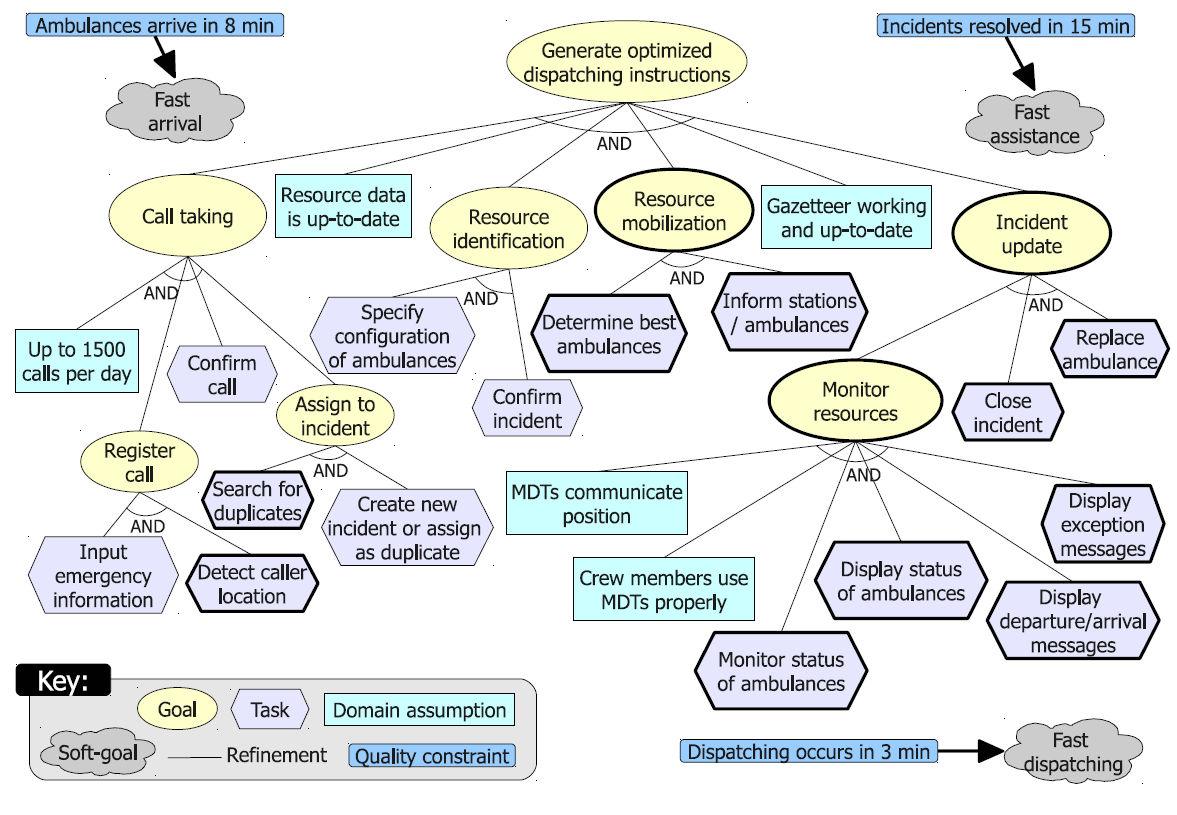
\includegraphics[width=1\textwidth]{figuras/modelos/ACAD-Simples.png}
	\caption{Exemplo de modelos de objetivos ~\cite{tesevitor}}
	\label{figura-acad-simples}
\end{figure}

% ======================================================================================================
% SUBSEÇÃO Modelos de Objetivos em Tempo de Execução
% ======================================================================================================

\subsection{Modelos de Objetivos em Tempo de Execução}
\label{sec-referencial-engenharia-objetivos-runtime}

% Sistemas adaptativos
Muitas vezes os requisitos de um \textit{software} precisam ser modificados durante o ciclo de execução do mesmo. Além disso, durante o processo de especificação as partes interessadas no sistema podem apresentar requisitos condicionais, ou seja, que assumem diferentes configurações dependendo da ocorrência de determinada situação~\cite{souza2012requirement}. Em outras palavras, há a necessidade de sistemas que possam se automonitorar e, caso necessário, se adaptarem para que seus objetivos continuem sendo satisfeitos~\cite{dalpiaz2013runtime}. Esse tipo de sistema geralmente é composto por duas partes principais: a primeira sendo o sistema em si, que executa uma tarefa para cumprir um objetivo desejado e a segunda sendo um sistema de monitoramento do primeiro, que envia ao primeiro sistema instruções de modificação de suas configurações para que seus objetivos continuem sendo atendidos~\cite{souza2013awareness}. 

O sistema de monitoramento é construído fundamentado na premissa de que todo sistema possui um ciclo de retroalimentação (\textit{(feedback loop)})~\cite{brun2009engineering}, e assim realizam o processo de adaptação com base nesse ciclo, aplicando controladores de \textit{feedback} que monitoram o comportamento do sistema e injetam estratégias de adaptação~\cite{souza2013awareness}. O módulo adaptador do sistema verifica, de acordo com as saídas do sistema alvo, se os objetivos internos a esse estão sendo atendidos e, para isso, necessita importar o modelo de objetivos~\cite{souza2013awareness} enriquecido de elementos que indicam os requisitos a serem observados e as estratégias de adaptação relativas.

Modelos de sistemas adaptativos incluem requisitos autoconscientes, ou seja, requisitos definidos em relação ao sucesso, falha ou qualidade de serviço de outros requisitos~\cite{souza2013awareness}. Assim, esses requisitos são considerados ``requisitos especiais'' já que sua operacionalização está relacionada a mudança de outros requisitos~\cite{souza2012requirement}. Ademais, o comportamento do sistema é caracterizado por eventos que ocorrem em tempo de execução e que estão diretamente ligados a instâncias de objetivos~\cite{dalpiaz2013runtime}. Assim, é importante observar que essa abordagem é considerada orientada a objetivos já que os requisitos mencionados são derivados do refinamento de objetivos elicitados para o sistema.

%Awreqs
Requisitos autoconscientes são divididos em dois tipos principais: Requisitos de Percepção (\textit{Awareness Requirements} ou \awreqs)~\cite{souza2013awareness} e Requisitos de Evolução (\textit{Evolution Requirements} ou \evoreqs)~\cite{souza2012requirement}. \awreqs são requisitos que referem-se ao estado de outros requisitos em tempo de execução, representando situações onde as partes interessadas desejam que o sistema se adapte~\cite{souza2012requirement}. Podem se referir a qualquer tipo de elemento, sejam objetivos, \sofgoals, tarefas e pressuposições de domínio. Além disso, indicam o quão critico um requisito pode ser ao descrever o grau de tolerância a falhas do mesmo~\cite{souza2012requirement}. Antes da execução de um sistema, os requisitos estão em estado ``Não Decidido'' (\textit{undecided}), e então pode assumir os estados ``Sucesso'' (\textit{Succeeded}), ``Falha'' (\textit{Failed}), e no caso de objetivos e tarefas, ``Cancelado'' (\textit{Canceled})~\cite{souza2013awareness}. É facilmente notável que o processo de elicitação de requisitos de percepção só acontece depois que o modelo de objetivos é levantado, e assim como o processo de construção de objetivos, \awreqs devem ser sistematicamente criados.

%Evoreqs
\evoreqs são requisitos que modificam o espaço de comportamento do sistema, permitindo que novas alternativas de requisitos sejam usadas, baseando-se em um conjunto pré-definido de etapas de evolução para os requisitos monitorados~\cite{souza2012requirement}. Isto é, \evoreqs são requisitos que especificam uma série de operações primárias em relação a outros requisitos diante de determinadas situações, dizendo ao sistema como adaptar-se~\cite{souza2012requirement}, como por exemplo, adicionar ou remover um objetivo, modificar o estado de um objetivo (em nível de instância), desfazer as ações de uma execução que resultou em falha, entre outras~\cite{souza2013requirements}.

Em suma, \awreqs especificam quando um determinado objetivo precisa de mudanças para continuar a ser atendido, enquanto \evoreqs especificam como executar tais mudanças. A seguir, o modelo de exemplo apresentado na seção~\ref{sec-referencial-engenharia-objetivos} é novamente apresentado, porém com novos requisitos de adaptação que são devidamente discutidos na próxima sessão.

% ======================================================================================================
% SUBSEÇÃO Exemplo de Caso de Uso
% ======================================================================================================
\subsection{Exemplo de Modelagem de Caso de Uso}
\label{sec-referencial-engenharia-objetivos-exemplo}

Na Figura~\ref{figura-acad-completo} é apresentado o modelo completo do sistema de despacho de ambulâncias (\textit{Adaptive Computer-aided Ambulance Dispatch} ou \textit{A-CAD}), nele observa-se o objetivo principal ``Gerar Instruções de Despacho Otimizadas'', representado por uma oval, que é imediatamente refinado em outros objetivos e em uma pressuposição de domínio (retângulo), o refinamento entre o objetivo raiz e seus filhos imediatos é do tipo ``E'' e portanto, para que o objetivo principal seja considerado satisfeito, todos as suas decomposições de primeiro grau precisam ser satisfeitas. Então, verifica-se que o primeiro nível de refinamento do objetivo principal é composto de:

\begin{itemize}
	\item Objetivo: ``Gerenciar Chamadas''
	\item Objetivo: ``Identificação de Recursos''
	\item Objetivo: ``Mobilização de Recursos''
	\item Objetivo: ``Obtenção de Mapas''
	\item Pressuposição de Domínio: ``Dados sobre recursos está sempre atualizado''
\end{itemize}

\begin{figure}[h]
	\centering
	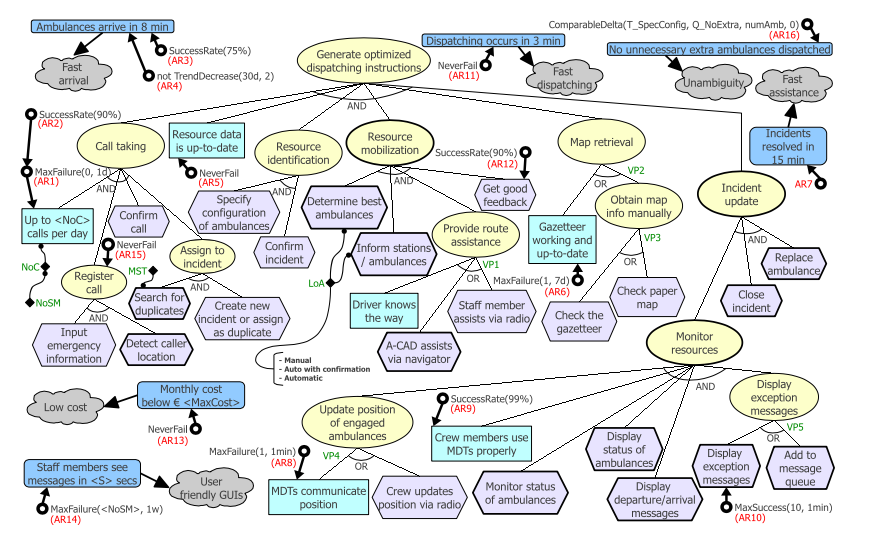
\includegraphics[width=1\textwidth]{figuras/modelos/ACAD-Completo.png}
	\caption{Exemplo de modelos de objetivos de um sistema de despacho de ambulâncias ~\cite{tesevitor}}
	\label{figura-acad-completo}
\end{figure}

O processo de refinamento do modelo então segue até que todos os objetivos sejam completamente refinados em tarefas ou pressuposições de domínio. \sofgoals são representados por nuvens e refinados em critérios de operacionalização representados por retângulos com cantos arredondados. Exemplificando, o \sofgoal ``Chegada Rápida''é operacionalizado por ``Ambulâncias chegam em oito minutos'', assim, tem-se um critério claro de satisfação para um objetivo que antes possuía diversos tipos de interpretação, porém agora, sabe-se que uma ambulância chega rapidamente se consegue estar no local do acidente em menos de oito minutos a partir da chamada.

Os requisitos de percepção são representados por um círculo oco. Por exemplo, o \awreq identificado por ``AR15'', indica que o objetivo ``Registrar Chamados'' deve ``Nunca falhar''. Os \evoreqs referentes a cada um dos \awreqs não são representados nesse modelo, e devem ser especificados em forma de sequencia de operações sobre os elementos do modelo de objetivos (essa escolha visa aprimorar a legibilidade do modelo). Além dos \awreqs, são especificados também os parâmetros de controle (\textit{control parameters}), representados por losangos, que indicam parâmetros do sistema que podem ser reconfigurados durante a adaptação. Todas as formas de representação estão resumidas na Figura~\ref{figura-elementos-gore-eca}.

\begin{figure}[h]
	\centering
	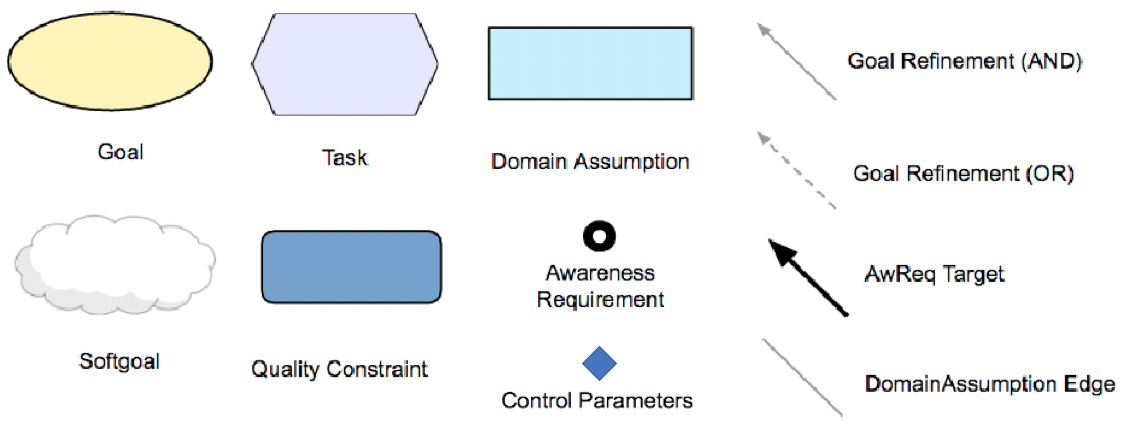
\includegraphics[width=1\textwidth]{figuras/modelos/Elementos-GORE.png}
	\caption{Representação gráfica de elementos de \gore}
	\label{figura-elementos-gore-eca}
\end{figure}

Sobre os \evoreqs do ``AR15'', podemos definir seus respectivos Requisitos de Evolução. Primeiramente, se o objetivo vir a falhar, define-se a primeira estratégia de adaptação como ``Tentar Novamente em 5 segundos no máximo uma vez'' (\texttt{RetryStrategy(5000)}), caso falhe mais do que uma vez, aplica-se outra estratégia ``Diminuir Condições ao Desabilitar Filho'' (\texttt{RelaxDisableChild(TDetectCaller)}), que desativa o requisito ``Detectar Localização da Ligação'', também aplicado no máximo uma vez. Essas decisões são sumarizadas na tabela \ref{tabela-evoreqs-ar15}.

\begin{table}[]
	\centering
	\caption{Tabela de especificação das estratégias de adaptação de AR15.}
	\label{tabela-evoreqs-ar15}
	\begin{tabular}{lll}
		AR15 & NeverFail(G\_RegCall) & \begin{tabular}[c]{@{}l@{}}1. Retry(5000)\\ 2. RelaxDisableChild(T DetectCaller)\end{tabular}
	\end{tabular}
\end{table}

O processo de especificação de como as estratégias de evolução são realizadas pelo sistema é discutido na próxima seção.

% ======================================================================================================
% SEÇÃO Zanshin
% ======================================================================================================

\section{Zanshin}
\label{sec-referencial-zanshin}

Apresentado por~\cite{tesevitor} e baseado em várias das premissas discutidas até aqui, \zanshin é um \textit{framework} que utiliza de ciclos de retro-alimentação para monitorar sistemas e enviar estratégias de adaptação com base em informações de modelos de requisitos orientados a objetivos enriquecidos com elementos como os \awreqs e os \evoreqs. O nome \zanshin vem de um termo usado em artes marciais japonesas e significa estado de completa consciência.

Em tempo de execução, os elementos do modelo de objetivos são representados por classes e instanciados cada vez que o usuário (ou sistema) busca atingir um objetivo, e então o sistema passa a enviar mensagens a essas instâncias quando detectar falhas. Percebe-se assim, que objetivos e pressuposições de domínio não são tratadas como invariantes que devem sempre ser atingidas, já que o sistema pode falhar ao tentar atingir seus objetivos iniciais, e assim o sistema de adaptação lidará com essas falhas e tomará medidas para que os objetivos voltem a ser satisfeitos~\cite{souza2013requirements}.

Assim como o monitoramento de objetivos através do \textit{Feddback Loop}, o \zanshin também monitora Parâmetros (\textit{Parameters}) que podem ser definidos em dois tipos. Primeiro, os Pontos de Variação (ou \textit{Variation Points}), que representam refinamentos do tipo ``OU'' (\textit{OR}). Por exemplo, o VP4 do modelo de objetivos do sistema A-CAD (Figura~\ref{figura-acad-completo}) que refere-se ao objetivo ``Atualizar posição de ambulâncias em uso'' especifica que atualizações de posição das ambulâncias podem ser obtidas automaticamente ou via rádio. Segundo, as Variáveis de Controle (ou \textit{Control Variables}), que são abstrações referentes a pontos de variação repetitivos ou usados em grande escala, como por exemplo a variável MST (``Tempo de Busca Mínimo'' ou \textit{Minimum Search Time}), que refere-se a tarefa ``Procurar por (incidentes) duplicados''.

O metamodelo dos modelos de objetivos usados no \zanshin é representado na Figura~\ref{figura-metamodelo-antigo}, e especificado no código do \textit{framework} como um modelo \emf e carregado em memória como objetos \java usando a API do \eclipse para \emf. Nessa caso, o modelo \emf representa os tipos de requisitos em nível de classe~\cite{souza2013requirements}. 

\begin{figure}[h]
	\centering
	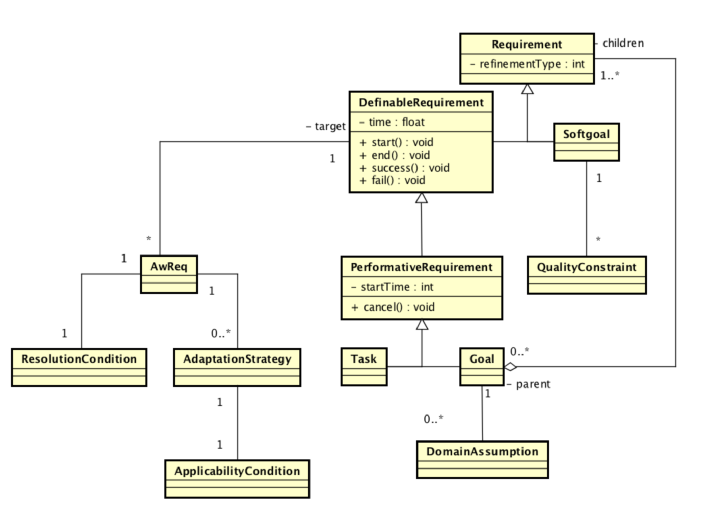
\includegraphics[width=1\textwidth]{figuras/metamodelos/metamodelo-zanshin-antigo.png}
	\caption{Metamodelo que define a sintaxe abstrata para o \zanshin}
	\label{figura-metamodelo-antigo}
\end{figure}

De uma maneira geral, o \zanshin é ser divido em quatro componentes. Essa seção discute dois módulos principais: o componente de monitoramento e o componente de adaptação.

% ======================================================================================================
% SUBSEÇÃO Zanshin: Monitoramento
% ======================================================================================================
\subsection{Monitoramento}
\label{sec-referencial-zanshin-monitoramento}

O módulo de monitoramento necessita que o sistema alvo implemente funcionalidades de registro (\textit{logs}). Através do registro, o sistema pode detectar mudanças nos estados das instâncias de um \awreq e assim notificar o serviço de adaptação sobre as mudanças ocorridas. 

Para identificar o modelo de objetivos do sistema alvo, o componente de monitoramento necessita da especificação do modelo do sistema também em \emf. Através dele, o \zanshin criará instancias desses objetivos extendendo as de classes carregadas do metamodelo de \gore referentes ao tipo de cada um deles. Ou seja, o modelo do sistema deve especificar objetos que extendam os disponíveis no metamodelo de \gore (Figura~\ref{figura-metamodelo-antigo}). Por exemplo, ao criar tarefa ``Especificar configuração de ambulâncias'', o sistema criará uma instancia dessa tarefa específica, que fará referência a classe \texttt{Task} criada no momento em que o metamodelo foi importado. A classe de tarefa especializa a classe \texttt{PerformativeRequirement} que é uma especialização \texttt{DefinableRequirement}. 

\textit{Performative Requirements} definem os tipos de requisitos que são ou podem ser refinados em tarefas, e assim possuem ações que são executadas pelo sistema ou seus usuários. Enquanto \textit{Definable Requirements} são os requisitos que deve possuir um estado definido em algum momento da execução, como por exemplo os objetivos e pressuposições de domínio.

Assim que o sistema cria as classes dos requisitos do sistema alvo, o processo de monitoramento apoia nos métodos definidos nas metaclasses \texttt{DefinableRequirement} e \texttt{PerformativeRequirement}~\cite{tesevitor} para realizar a monitoração, os métodos disponíveis são:
\begin{itemize}
	\item \texttt{start()}: esse método é chamado nas classes de critérios de qualidade e pressuposições de domínio imediatamente antes da análise de seu estado de satisfação. Para o caso de tarefas, esse método é chamado assim que um usuário inicia uma tarefa, e então todos os ancestrais a essa também tem esse método invocado.
	\item \texttt{sucess()}: chamado quando um requisito é satisfeito e propagado para todos os acentrais a esse objetivo para ``avisar'' que o filho chegou ao estado de sucesso.
	\item \texttt{fail()}: segue a mesma lógica dos item anteriores, propagando a ``falha'' de um requisito aos seus ancestrais.
	\item \texttt{cancel()}: para o caso de requisitos como objetivos e tarefas, esse método é usado quando um procedimento é cancelado pelo usuário, e usa da mesma lógica de propagação dos métodos anteriores para informar o ocorrido aos pais.
	\item \texttt{end()}: chamado assim que um requisito retorna dos estados de sucesso, falha ou cancelamento.
\end{itemize}

Através da descrição dos métodos acima mencionados, é possível entender como o processo de monitoramento funciona: basicamente os requisitos monitorados possuem métodos que podem ser chamados em cada caso que assumem, seja de sucesso, falha o ou cancelamento. Assim que chamados, os métodos invocam os mesmos métodos nos elementos pais, permitindo que a atualização de um requisito se propague a todos os elementos que interessem, atualizando assim todo o modelo.

Logo que o componente monitor detecta uma mudança de estado em um requisito, ou seja, assim que qualquer um dos métodos acima é invocado, ele imediatamente envia uma notificação sobre essa mudança ao módulo de adaptação, que então inicia o processo definido para aquele determinado requisito de percepção ~\cite{tesevitor}.

\subsection{Adaptação}
\label{sec-referencial-zanshin-adaptacao}
Em termos de implementação, o algoritmo do módulo de adaptação cria uma sessão para cada \awreq que está sendo monitorado e então gera uma fila de eventos que se referem a estratégias de adaptação. Assim, essa linha de eventos pode ser usada para verificar se uma estratégia é ou não aplicável a determinada situação. Primeiramente, deve-se verificar o estado de um objetivo apontado por um \awreq, para isso é checada a condição de resolução daquele. Então, caso uma avaliação considere que o objetivo está em estado de falha, o sistema segue (seguindo uma ordem pré-definida) a lista de estratégias de adaptação disponíveis, procurando alguma que tenha sua condição de aplicabilidade verdadeira. Caso encontre, aplica a estratégia de adaptação definida por aquela condição de aplicabilidade e então retorna ao estado inicial, onde a checagem da satisfabilidade do objetivo é realizada novamente. Caso o sistema retorne a fase de checagem do estado do objetivo e esse ainda não tenha sido satisfeito, o processo começa novamente. Caso não encontre uma condição para aplicar uma estratégia, o sistema ativa o método ``abortar'' (\texttt{abort()})~\cite{souza2013requirements}. 

Ao final, quando uma sessão de adaptação é considerada resolvida, a mesma deve ser terminada e se for necessário que o processo seja aplicado novamente, uma nova sessão é criada. Entretanto, se uma sessão termina sem ter resolvido o problema, o \textit{framework} continuará trabalhando nela do ponto em que parou assim que receber uma nova requisição para adaptação daquele mesmo \awreq. Porém, algumas estratégias também podem forçar que a sessão seja reiniciada quando executada ~\cite{souza2013requirements}. Essa processo é conhecido como Evento de Ação-Condição (\textit{Event Condition Action} ou \textit{ECA}) ~\cite{morin2009models}.

\subsubsection{ECA}
\label{sec-referencial-zanshin-eca}

O código a seguir resume o processo \textit{ECA} para realizar a seleção de estratégias de adaptação:

\begin{lstlisting}[caption={Código do processo ECA},label={listagem-estrategias-AR15}]
processEvent(ar : AwReq) {
	session = findOrCreateSession(ar.class);
	session.addEvent(ar);
	solved = ar.condition.evaluate(session);
	if(solved) break;

	ar.selectedStrategy = null;
	for each s in ar.strategies {
		appl = s.condition.evaluate(session);
		if (appl) {
			ar.selectedStrategy = s;
			break ;
		}
	}

	if (ar.selectedStrategy == null)
		ar.selectedStrategy = ABORT;

	ar.selectedStrategy.execute(session);
	ar.condition.evaluate(session);
}
\end{lstlisting}

O algoritmo incia obtendo a sessão de adaptação referente a classe do \awreq requisitado (caso não haja uma sessão, uma nova é criada). Obtida a sessão de adaptação, o algoritmo tem então acesso a lista de eventos de aplicabilidade referentes, então, adiciona o \awreq a sessão e imediatamente verifica o estado da mesma (verificando a condição de resolução), parando caso tenha retornado estado de sucesso. Caso contrário, o processo continua procuando por uma estratégia que seja aplicável, verificando se a condição de aplicabilidade é verdadeira. Caso for verdadeira, interrompe o processo e dá a sessão de adaptação uma nova chance de verificar o estado do \awreq. Caso todas as condições sejam falsas e nenhuma estratégia seja selecionada, seleciona a estratégia padrão (\texttt{abort()}) e termina o processo~\cite{tesevitor}. 

Para exemplificar esse processo, tomemos novamente o \awreq ``AR15'', que garante que o requisito ``Registrar chamada'' deve nunca falhar. Caso seja detectado pelo processo de monitoramento que esse requisito apresenta estado de falha, o módulo monitor imediatamente ativa o módulo de adaptação, que segue o processo ECA para aplicar estratégias ao ``AR15''. Pela Listagem~\ref{listagem-estrategias-AR15}, ve-se que a condição de resolução desse requisito é do tipo \texttt{SimpleResolutionCondition} e que a primeira estratégia a ser selecionada é \texttt{RetryStrategy}, ou seja, tentar novamente (em 5s), entretanto, essa estratégia possui a condição de aplicabilidade \texttt{MaxExecutionsPerSessionApplicabilityCondition}, o que significa que ela só pode ser aplicada uma vez naquela sessão. Caso essa condição seja falsa, a próxima estratégia refere-se a desativar um dos filhos desse objetivo (\texttt{RelaxDisableChildStrategy}), no caso a tarefa ``Detectar localização da chamada'', e possui a mesma condição de aplicabilidade. Se nenhuma dessas condições puder ser satisfeitas, então o sistema aborta, caso contrário, seleciona a primeira estratégia aplicável e verifica novamente o estado do objetivo. A condição \texttt{SimpleResolutionCondition} refere-se ao fato de que um objetivo é dito satisfeito apenas se seus filhos estiverem em estado de sucesso (respeitando a regra booleana do refinamento). 

\begin{lstlisting}[caption={Estratégias de adaptação de AR15},label={listagem-estrategias-AR15}]
<awreqs xsi:type="acad:AR15">										
	<condition xsi:type="eca:SimpleResolutionCondition"/>
		<strategies xsi:type="eca:RetryStrategy" time="5000">
			<condition xsi:type="eca:MaxExecutionsPerSessionApplicabilityCondition" maxExecutions="1"/>
		</strategies>
		<strategies xsi:type="eca:RelaxDisableChildStrategy" child="//@rootGoal/@refinements.0/@refinements.0/@refinements.1">
			<condition xsi:type="eca:MaxExecutionsPerSessionApplicabilityCondition" maxExecutions="1"/>
		</strategies>
</awreqs>
\end{lstlisting}

É importante salientar que as classes referentes a estratégias de adaptação, assim como as condições de aplicabilidade e resolução podem ser extendidas para casos mais complexos, envolvendo inclusive a interação humana ~\cite{tesevitor}.

%For example, the trivial case is considering the problem solved if the (next) AwReq evaluates to success, but this abstract class can be extended to provide di↵erent kinds of resolution conditions, including, e.g., involving a human-in-the-loop to confirm if the problem has indeed been solved, organizing conditions into AND/OR-refinement trees (like in a goal model), etc.

% ======================================================================================================
% SUBSEÇÃO DESENVOLVIMENTO ORIENTADO A MODELOS
% ======================================================================================================
\section{Desenvolvimento Orientado a Modelos}
\label{referencial-mdd}
Pesquisadores vem tentando ao longo dos anos criar abstrações que ajudem programadores a focar no conteúdo do desenvolvimento ao invés das especifidades da tecnologia de criação adotada~\cite{viyovic2014sirius}. O Desenvolvimento Orientado a Modelos  pode ser visto como a forma de programação de mais alto nível de abstração existente atualmente~\cite{atkinson2003model}, promovendo o uso de artefatos do processo de desenvolvimento de software para lidar com complexidade através de abstração~\cite{viyovic2014sirius}. Em outras palavras, MDD parte da premissa que um sistema é um modelo consistente com seu metamodelo~\cite{vujovic2014comparative}, assim, em vez de exigir que programadores escrevam cada simples detalhe da implementação de um sistema, permite que uma funcionalidade necessária para um software pode ser visualmente modelada ~\cite{atkinson2003model}. Sendo assim, essa técnica viabiliza que muitas atividades complexas (porém rotineiras) sejam automatizadas na área de programação de software, como por exemplo o suporte a persistência, interoperabilidade e distribuição ~\cite{atkinson2003model}.

A modelagem usa da percepção visual humana para melhorar o processo de compreensão sobre o domínio de um software, já que modelos nos auxiliam a entender problema complexos e suas possíveis soluções através da abstração. Assim, MDD baseia-se na premissa de que o desenvolvimento de software deve focar principalmente na produção de modelos e não na criação de código ~\cite{selic2003pragmatics}. A primeira vantagem dessa abordagem é que podemos usar conceitos mais ligados ao domínio do problema que software vai resolver do que conceitos técnicos ligados a linguagem de programação. Essa vantagem acarreta em alguns outros benefícios: modelos são mais compreensíveis do que códigos e portanto, tornam-se também mais fáceis de especificar e manter~\cite{selic2003pragmatics}. Além disso, modelos são menos sensíveis a alterações de tecnologias, ou seja, são independentes de plataforma~\cite{selic2003pragmatics}. Em conclusão, observa-se que o principal (porém não único) aspecto de MDD é a produção automática de código através da interpretação de modelos visuais~\cite{selic2003pragmatics, viyovic2014sirius}.

\subsection{Eclipse Modeling Framework}
O \eclipse é um projeto de código aberto com o objetivo de prover uma plataforma de desenvolvimento altamente integrada. O processo de criação de sistemas no \eclipse pode ser divido em alguns projetos, entre eles o Projeto de Modelagem (\textit{Modeling Project}), que foca em tecnologias baseadas no desenvolvimento orientado a modelos~\cite{steinberg2008emf}. Esse ambiente é chamado de \textit{Eclipse Modeling Framework} ou \textit{EMF}, e provê funcionalidades como transformação de modelos, integração de bases de dados e geração de editores gráficos~\cite{steinberg2008emf}. Modelos especificados através de \emf relacionam conceitos de modelagem diretamente a seus conceitos de implementação, sendo a união das tecnologias \uml, \xml e \java, permitindo a conversão automática entre todas essas ferramentas~\cite{steinberg2008emf}. 

A tecnologia \emf pode ser melhor explicado com um exemplo: um sistema de gerenciamento de ordem de compras de uma loja, que necessite incluir casos como ``cobrar'' e ``entregar'' em um endereço, e uma coleção de itens (nesse caso compras). A figura~\ref{exemplo-uml} mostra o diagrama em \uml do sistema. Esse modelo pode também ser descrito dentro do \emf usando modelos \ecore, como na Figura~\ref{exemplo-ecore}. Modelos \ecore são basedos no metamodelo para especificação exibido na Figura~\ref{metamodelo-ecore}, onde classes são representadas por \texttt{EClass}, atributos por \texttt{EAttribute}, relações por \texttt{EReference} e tipos de dados por \texttt{EDataType}. Assim, a ``conversão'' do modelo \uml para \ecore é dada ao se instanciar classes de \ecore de acordo com a especificidade do domínio do problema, como pode ser visto na Figura~\ref{exemplo-uml-to-ecore}~\cite{steinberg2008emf}. 

\begin{figure}[h]
	\centering
	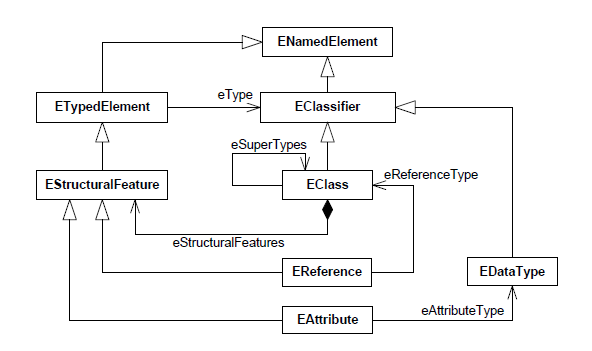
\includegraphics[width=0.95\textwidth]{figuras/exemplos-emf/metamodelo-ecore.png}
	\caption{Metamodelo de \ecore~\cite{kern2008interchange}}
	\label{metamodelo-ecore}
\end{figure}

\begin{figure}[h]
	\centering
	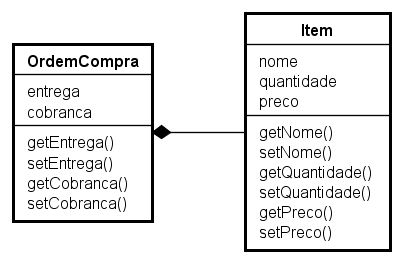
\includegraphics[width=0.65\textwidth]{figuras/exemplos-emf/exemplo-uml.png}
	\caption{Classes do diagrama do exemplo em \uml}
	\label{exemplo-uml}
\end{figure}

\begin{figure}[h]
	\centering
	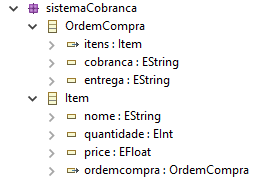
\includegraphics[width=0.7\textwidth]{figuras/exemplos-emf/exemplo-ecore.PNG}
	\caption{Classes do diagrama do exemplo em \ecore}
	\label{exemplo-ecore}
\end{figure}

Assim que o modelo é detalhado em \ecore, o \emf está pronto para gerar código automaticamente, seguindo os seguintes passos:

\begin{itemize}
	\item Para cada tipo \texttt{EClass} são criadas uma interface e a classe de implementação correspondente. Então para o exemplo de classe \texttt{OrdemCompra} serão criadas a interface \texttt{OrdemCompra} e a classe \texttt{OrdemCompraImpl}. Essa especificação permite que sejam implementadas funções de persistência e distribuição, porém não serão discutidas aqui por fugirem do escopo desse trabalho.
	\item As classes do tipo \texttt{EAtributte} são transformadas em atributos nas classes correspondentes
	\item As classes tipo \texttt{EReference} são transformadas em referências nas respectivas classes as quais referenciam.
\end{itemize}

\begin{figure}[h]
	\centering
	
\includegraphics[width=1\textwidth]{figuras/exemplos-emf/uml-to-ecore.png}
	\caption{Conversão do diagrama de exemplo de \uml para \ecore}
	\label{exemplo-uml-to-ecore}
\end{figure}

Em suma, o \framework de modelagem do \eclipse permite que usuários criem modelos apoiados em metamodelos, e baseando-se no modelo criado, gerem partes de código de sistema~\cite{vujovic2014comparative}.

%https://books.google.com.br/books?id=sA0zOZuDXhgC&lpg=PT23&ots=2IQIWZWqNm&dq=eclipse&lr&hl=pt-BR&pg=PT45#v=onepage&q=eclipse&f=false

\subsection{Sirius}

O \sirius é um plugin que simplifica o \framework de Modelagem Gráfica (\textit{Graphical Modeling Framework} ou \textit{GMF}) do \eclipse, reduzindo a complexidade de uso do mesmo e permitindo a produção de editores gráficos de modelos personalizados~\cite{viyovic2014sirius}. O \sirius é construído em cima do fato de que o \eclipse provê utilidades para (des)serialização de modelos, checagem de condições e geração de editores baseados em \emf~\cite{budinsky2004eclipse}. Representações criadas com \sirius podem ser apresentadas em diagramas, tabelas e árvores~\cite{viyovic2014sirius}. Em síntese, \sirius provê ferramentas que permitem a especificação de um modelo de um domínio qualquer em diferentes perspectivas~\cite{vujovic2014comparative}.

Através de modelos de especificação (\textit{Viewpoint Specification Model} ou VSM), o \textit{plugin} permite especificar a estrutura, aparência e comportamento do metamodelo do editor a ser criado~\cite{viyovic2014sirius}. Os VSMs são especificados através de arquivos \textit{.odesign}~\cite{viyovic2014sirius}, e baseam-se na especificação do metamodelo em \ecore. Um exemplo de caracterização de representação de modelos é mostrado na figura~\ref{exemplo-sirius} retirada de~\cite{viyovic2014sirius}.

\begin{figure}[h]
	\centering
	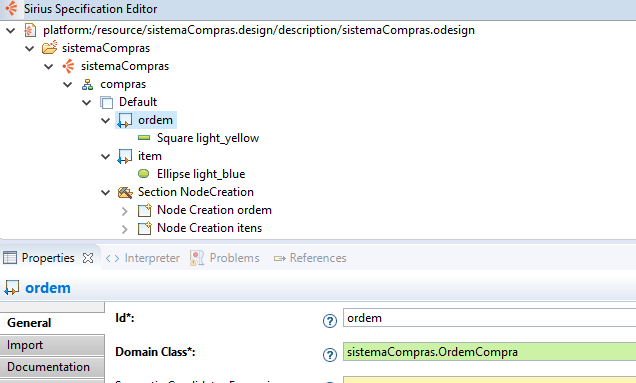
\includegraphics[width=0.9\textwidth]{figuras/exemplos-emf/exemplo-sirius-vsm.png}
	\caption{Exemplo de \textit{Viewpoint Specification Model}}
	\label{exemplo-sirius}
\end{figure}

\sirius provê vários mecanismos que auxiliam no gerenciamento da complexidade de modelos~\cite{madiot2015eclipse}:

\begin{itemize}
	\item \textbf{Camadas}: é possível separar elementos em camadas diferentes, e ativar ou desativar essas.
	\item \textbf{Filtros}: exibir ou esconder elementos dependendo de determinada condição.
	\item \textbf{Fersonalização de Estilos}: permite modificar propriedades gráficas de elementos do diagrama.
	\item \textbf{Regras de Validação}: permite que a qualidade do modelo seja avaliada.
\end{itemize}


% ==============================================================================
% TCC - César Henrique Bernabé
% Capítulo 3 - O Unagi
% ==============================================================================

\chapter{Especificação de Requisitos}
\label{sec-unagi}

Este capítulo aborda alguns resultados da Engenharia de Requisitos para a construção do sistema SAE. Na seção~\ref{sec-requisitos-escopo}, é apresentado o escopo do projeto; na seção~\ref{sec-requisitos-casos-de-uso}, são apresentados diagramas de casos de uso e na seção~\ref{sec-requisitos-diagrama-de-classes}, são apresentados os diagramas de classes. Os requisitos funcionais, requisitos não funcionais e regras de negócio podem ser encontrados no \textbf{Documento de Especificação de Requisitos} que está disponível no Apêndice ao final desta monografia.


\section{Descrição do Escopo}
\label{sec-requisitos-escopo}

O DI/Ufes deseja um sistema de informação para acompanhar seus alunos egressos dos cursos de graduação (Ciência da Computação e Engenharia de Computação) e de pós-graduação (Mestrado em Informática e Doutorado em Ciência da Computação). 

Para poder acessar o sistema, os egressos terão um pré-cadastro realizado por um administrador do sistema. Somente poderão ser pré-cadastrados ex-alunos que tenham se formado em algum curso oferecido pelo DI/Ufes. Para efetuar o pré-cadastro o administrador buscará os dados do egresso junto à Ufes, a saber: nome, data de nascimento, sexo, e-mail, identidade, CPF, naturalidade e nacionalidade. Também serão informados o curso em que o egresso se formou, o número de sua matrícula, o ano de ingresso e o ano de término. 

Assim que o pré-cadastro for realizado, o sistema deverá enviar um e-mail ao egresso com um link que o leva diretamente para uma página onde pode definir sua senha. Para aumentar a segurança, esta página solicita o CPF ou a matrícula do egresso para efetivar a definição de senha. Caso o egresso perca este e-mail, poderá receber outro, devendo para isso entrar no site e informar o seu CPF/matrícula. Reconhecendo o egresso, o sistema enviará o e-mail.
 
Assim que for criada a senha, o sistema levará o egresso a uma página onde ele preencherá um formulário com os seguintes campos: faixa salarial, área de atuação, se atua na área em que se formou, nível de escolaridade e se reside no ES. Para cada nível de escolaridade deve dizer o título obtido, o ano, a instituição, o estado e o país.

O tempo médio exigido para o preenchimento deste formulário deve ser inferior a 5 minutos. A cada 2 anos o sistema deverá enviar um e-mail para que o usuário atualize esses dados, sendo armazenado o histórico dos mesmos.

Os egressos escolherão a sua área de atuação dentre as seguintes opções: empreendedor; funcionário público; funcionário privado; professor; ou pesquisador. E informarão se atuam em Informática, área afim ou área não correlata. Será perguntado se a formação acadêmica adquirida no curso da Ufes contribuiu para a sua atividade atual.

Os egressos escolherão a faixa salarial, dividida da seguinte forma: até 3 salários mínimos; de 3 a 5 salários mínimos; de 5 a 10 salários mínimos;  de 10 a 15 salários mínimos; de 15 a 20 salários mínimos; e acima de 20 salários mínimos. Poderão também optar por assuntos de interesse para recebimento de e-mail. A princípio os assuntos serão: Redes de Computadores e Sistemas Distribuídos; Computação de Alto Desempenho; Inteligência Computacional; Sistema de Informação; e Otimização. 

Egressos poderão postar depoimentos sobre o curso que realizaram. Esses depoimentos ficarão acessíveis a todos que acessarem o site, depois de serem avaliados e liberados pelo coordenador do curso a fim de evitar críticas gratuitas depreciativas. O egresso poderá optar por aparecer seu nome no depoimento ou se ele quer que fique anônimo. De um depoimento deseja-se saber a data de envio, sobre qual curso, o autor e o conteúdo. 

Assim como no caso dos depoimentos, os egressos também poderão mandar comentários ou sugestões sobre o curso que realizaram. Estes serão enviadas para o coordenador do curso para que possa respondê-los e também auxiliar em melhorias a serem feitas nos cursos. 

Administradores do sistema poderão cadastrar seminários, informando o assunto, o título, a data e horário, o local e o palestrante. Caso não tenha palestrante ainda, o administrador terá a opção de enviar um e-mail aos egressos convidando-os a serem o palestrante. Caso alguém responda ao chamado (por e-mail, externo ao sistema), o administrador terminaria o cadastro do seminário. Assim que a palestra estiver confirmada, o sistema enviará um e-mail para todos os egressos que tenham interesse pelo assunto, convidando-os para participarem. Os egressos também teriam a opção de sugerir um assunto em que tenham interesse em ser o palestrante. Neste caso o administrador confirmaria com ele e cadastraria o seminário no sistema.


No site, ficarão disponíveis para consulta relatórios sobre dados estatísticos. Estes dados serão mostrados na forma de gráficos, assim os usuários poderão escolher um curso e optar pelos seguintes gráficos: 

\begin{itemize}
	
  	\item \textbf{Faixa Salarial:} mostra a porcentagem de egresso em cada faixa salarial.
  	
  	\item \textbf{Área de Atuação:} mostra a porcentagem de egresso em cada área: (Empreendedor), (Func. Público), (Func. Privado), (Professor) e (Pesquisador).
  	
  	\item \textbf{Atuação do Egresso:} mostra a porcentagem de egressos que atuam na área da informática, a porcentagem dos que atuam em áreas afins e a porcentagem dos que atuam em áreas não correlatas. 
  	
  	\item \textbf{Escolaridade:} mostra a porcentagem de egressos em cada nível de escolaridade. 
  	
  	\item \textbf{Reside no ES:} mostra a porcentagem de egressos que moram no Estado.
  	
  	\item \textbf{Sexo:} mostra a porcentagem de egressos do sexo masculino e feminino.
  	  	
\end{itemize}

Os usuários também poderão consultar todos os egressos, que serão mostrados na forma de lista. 











%%% Início de seção. %%%
\section{Diagrama de Casos de Uso}
\label{sec-requisitos-casos-de-uso}
	
Este projeto foi divido em dois subsistemas \texttt{sae.core} e \texttt{sae.public}, sendo que o subsistema \texttt{sae.core} envolve toda a funcionalidade relacionada com o administrador do sistema, abrangendo controle de seminários, cursos, assuntos de interesse, envio de e-mail automático e pré-cadastro de egresso. O subsistema \texttt{sae.public} envolve toda a funcionalidade relacionada com consultas a serem realizadas no site, e com as interações que os egressos poderão fazer, tais como cadastrar depoimentos e sugestões.
Veremos na Subseção~\ref{sec-requisitos-casos-de-uso-core} os casos de uso do subsistema \texttt{sae.core} e na Subseção~\ref{sec-requisitos-casos-de-uso-public} os casos de uso do subsistema \texttt{sae.public}.
	
	
	
\subsection{Atores}
\label{sec-requisitos-casos-de-uso-atores}
O modelo de casos de uso visa capturar e descrever as funcionalidades que um sistema deve prover para os atores que interagem com o mesmo. A Tabela~\ref{tabela-atores} descreve cada um dos atores identificados no sistema.


	
\begin{table}[h]
	\centering \vspace{0.5cm} \caption{ Atores}
	\begin{tabular}{|p{3cm}|p{12cm}|} \hline \rowcolor[rgb]{0.8,0.8,0.8}
 		Ator & Descrição \\\hline                              
		Administrador & Profissional da Ufes responsável pela parte administrativa do sistema. \\\hline   
		Coordenador & É um administrador responsável por um curso, avaliando depoimentos e sugestões enviadas pelos egressos. \\\hline                              
		Egresso & Ex-alunos da Ufes que tenham se formado em algum curso oferecido pelo DI/Ufes. \\\hline                              
		Visitante & Qualquer pessoa que acessar o site. \\\hline 		 
	\end{tabular}
	\label{tabela-atores}	
\end{table}

	
A Figura~\ref{fig-requisitos-diagrama-atores} apresenta o diagrama de herança entre os atores do sistema, de modo que essas heranças não serão mostradas nos outros diagramas para evitar a poluição visual.
\begin{figure}[h]
	\centering
	\includegraphics[width=0.35\textwidth]{figuras/requisitos/atoresHeranca}
	\caption{SAE - CORE - Diagrama de Casos de Uso.}
	\label{fig-requisitos-diagrama-atores}
\end{figure}

	
\newpage	
\subsection{Subsistema sae.core}
\label{sec-requisitos-casos-de-uso-core}

A Figura~\ref{fig-requisitos-core-diagrama-casos-uso} mostra os casos de uso do subsistema \textbf{\texttt{sae.core}} que serão descritos a seguir. O subsistema \textbf{\texttt{sae.core}} foi criado para gerenciar as funcionalidades que só os administradores podem realizar. Os casos de uso \textbf{Gerenciar Cursos, Gerenciar Administradores, Gerenciar Egressos, Gerenciar Assuntos de Interesse e Gerenciar Seminário } são do tipo cadastrais e incluem alteração, inclusão, consulta e exclusão. 

\begin{figure}[h]
	\centering
	\includegraphics[width=0.95\textwidth]{figuras/requisitos/casodeuso-core}
	\caption{SAE - CORE - Diagrama de Casos de Uso.}
	\label{fig-requisitos-core-diagrama-casos-uso}
\end{figure}

O DI/Ufes possui cursos de graduação e de pós-graduação. Então, foi criado o caso de uso \textbf{Gerenciar Cursos} para que o administrador possa inserir novos cursos, possa também consultar, alterar e até mesmo excluir um curso. Para inserir um novo curso, basta informar o código, o nome e o coordenador do curso.

Uma informação crucial para o sistema são os Administradores, que serão controlados pelo caso de uso \textbf{Gerenciar Administradores}. Nesse caso, deve ser informado: nome, e-mail (será o login para acessar o sistema), CPF e matricula.

Os egressos são uma das partes fundamentais do sistema, assim serão controlados pelo caso de uso \textbf{Gerenciar Egresso}. As informações necessárias de um egresso são: nome, e-mail (será o login para acessar o sistema), data de nascimento, sexo, identidade, CPF, naturalidade e nacionalidade, também são necessários informar o curso, a matrícula, o ano de início e de término do curso.  

Os egressos poderão escolher assuntos de interesse para recebimento de e-mail. A princípio os assuntos serão: Redes de Computadores e Sistemas Distribuídos; Computação de Alto Desempenho; Inteligência Computacional; Sistema de Informação; e Otimização. Assim foi criado o caso de uso \textbf{Gerenciar Assuntos de Interesse} para realizar esse controle. A informação de um assunto é o nome.


Seminários também poderão ser cadastrados no sistema. Assim teremos os casos de uso \textbf{Gerenciar Seminário}, \textbf{Confirmar Seminário} e \textbf{Convidar Palestrante} para fazer o controle. O caso de uso  \textit{Gerenciar Seminário} será cadastral, enquanto o  \textit{Confirmar Seminário e Convidar Palestrante} envolve atividades como enviar e-mail a todos os egressos que tenham interesse no assunto do seminário assim que este for confirmado, enviar e-mail aos egressos convidando a serem o palestrante de seminário cujo assunto é de seu interesse.

Para manter os dados dos egressos atualizados será enviado, a cada 2 anos, um e-mail para todos os egressos solicitando que estes façam a atualização de seus dados. O caso de uso \textbf{Enviar e-mail atualizar dados} será responsável por este envio de e-mail.
	
	
	






\subsection{Subsistema sae.public}
\label{sec-requisitos-casos-de-uso-public}
 

A Figura~\ref{fig-requisitos-public-diagrama-casos-uso} mostra os casos de uso do subsistema \textbf{\texttt{sae.public}} que serão descritos abaixo. Este subsistema foi criado para gerenciar as funcionalidades relacionadas com consultas a serem realizadas no site e com as interações que os egressos poderão fazer, tais como cadastrar depoimentos e sugestões através dos casos de uso \textbf{Gerenciar Depoimentos, Gerenciar Sugestões, Gerenciar Escolaridades e Gerenciar Históricos}. Os casos de uso de consulta são \textbf{Consultar Todos Egressos, Consultar Depoimento e Consultar dados Estatísticos}, que poderão ser realizado por qualquer usuário do sistema. 

\begin{figure}[!h]
	\centering
	\includegraphics[width=1\textwidth]{figuras/requisitos/casodeuso-public}
	\caption{SAE - PUBLIC - Diagrama de Casos de Uso.}
	\label{fig-requisitos-public-diagrama-casos-uso}
\end{figure}

No caso de uso \textbf{Consultar Todos Egressos} as consultas poderão ser feitas de forma geral onde serão mostrados todos os egressos, ou por curso, onde serão mostrados apenas os egressos que formaram naquele curso. Será exibido na tela para ao usuário o nome do egresso, o curso que realizou, o ano de início e o ano de término.

No caso de uso \textbf{Consultar Depoimento} as consultas aos depoimentos poderão ser realizadas de forma geral onde serão mostrados todos os depoimentos, ou por curso, onde serão mostrados apenas depoimentos sobre o curso escolhido. Será exibido na tela o conteúdo, o autor e a data de postagem. Somente serão mostrados nesta consulta depoimentos que tenham sido analisados e aprovados pelo coordenador do curso que se refere o depoimento.

No caso de uso \textbf{Consultar dados Estatísticos} as consultas serão feitas com bases nos dados mais atuais dos egressos. Alguns exemplos de gráficos que poderão ser gerados nesta consulta são \textit{Faixa Salarial, Área de Atuação, Escolaridade e Sexo}.
  	  
Egressos poderão postar depoimentos sobre o curso que realizaram. Esses depoimentos ficarão acessíveis a todos que acessarem o site, depois de serem avaliados e liberados pelo coordenador do curso a fim de evitar criticas gratuitas depreciativas, assim foi criado o caso de uso \textbf{Gerenciar Depoimentos} para fazer esse controle.  

Assim como no caso dos depoimentos, os egressos também poderão mandar comentários ou sugestões sobre o curso que realizaram. Estes serão enviadas para o coordenador do curso para que possa respondê-los o caso de uso responsável por fazer esse controle é \textbf{Gerenciar Sugestões}.


No caso de uso \textbf{Gerenciar Históricos} o egresso informará sua faixa salarial, área de atuação que pode ser funcionário no setor público ou no setor privado, empreendedor, professor ou pesquisador, informará também se atua na área da informática, se reside no Espirito Santo e o seu maior nível de escolaridade. Com essas informações será possível criar o perfil dos egressos.


No caso de uso \textbf{Gerenciar Escolaridades} o egresso poderá cadastrar todos seus cursos realizados a nível de graduação, especialização, mestrado, doutorado ou pós-doutorado. Para cada curso ele informará a instituição, o estado e o país, e o ano de conclusão.


Maiores informações e detalhes sobre os casos de uso poderão ser consultados no \textbf{Documento de Análise de Requisitos} que está disponível no Apêndice ao final dessa monografia.






%%% Início de seção. %%%
\section{Diagrama de Classes}
\label{sec-requisitos-diagrama-de-classes}


Assim como os casos de uso na seção~\ref{sec-requisitos-casos-de-uso} os diagramas de classes estão dividos de acordo com a divisão dos subsistemas, na Subseção~\ref{sec-requisitos-diagrama-de-classes-core} estão as classes pertecentes ao subsistema \texttt{sae.core} e na Subseção~\ref{sec-requisitos-diagrama-de-classes-public} estão as classes pertencentes ao subsistema \texttt{sae.public}.



\subsection{Subsistema sae.core}
\label{sec-requisitos-diagrama-de-classes-core}

A Figura~\ref{fig-requisitos-core-diagrama-classes} exibe o diagrama de classes do subsistema \textbf{\texttt{sae.core}}. Uma das classes mais importante é a \textbf{Egresso} que possui ligações com outras classes tanto no subsistema \textit{\texttt{sae.core}} quanto no subsistema \textit{\texttt{sae.public}}. É obrigatório que um \emph{egresso} possua um \emph{curso}, que será feito através da classe \textbf{Curso Realizado} visto que para ser egresso do DI/Ufes é preciso ter realizado um curso. Entretanto é opcional um \emph{egresso} ter um \emph{assunto de interesse}, podendo ter mais de um.

\begin{figure}[h]
	\centering
	\includegraphics[width=1\textwidth]{figuras/requisitos/diagrama-classe-core}
	\caption{SAE - CORE - Diagrama de Classes.}
	\label{fig-requisitos-core-diagrama-classes}
\end{figure}

As classes \textbf{Administrador} e \textbf{Assunto de Interesse} podem ter registros no sistema e mesmo assim não estarem ligadas a nenhuma outra classe. Todo \emph{curso} deve ter um \emph{administrador} associado a ele, visto que este desempenhará o papel de coordenador do curso, sendo responsável por avaliar depoimento e responder sugestões do curso que coordena. Um \emph{seminário} precisa ter, obrigatoriamente, um \emph{assunto de interesse}.



\subsection{Subsistema sae.public}
\label{sec-requisitos-diagrama-de-classes-public}

A Figura~\ref{fig-requisitos-public-diagrama-classes} exibe o diagrama de classes do subsistema \textbf{\texttt{sae.public}}. Podemos notar que as classes \textbf{Egresso} e \textbf{Curso} foram referenciadas do subsistema \texttt{sae.core}. Portanto, fazem parte desse subsistema as classes \textbf{Depoimento}, \textbf{Sugestão}, \textbf{Escolaridade} e \textbf{Histórico do Egresso}. Uma \emph{escolaridade} e um \emph{histórico do egresso} devem estar associados a um \emph{egresso}. Um \emph{depoimento} e uma \emph{sugestão}, além de um \emph{egresso}, também devem ter um \emph{curso} associado a eles.

\begin{figure}[h]
	\centering
	\includegraphics[width=1\textwidth]{figuras/requisitos/diagrama-classe-public}
	\caption{SAE - PUBLIC - Diagrama de Classes.}
	\label{fig-requisitos-public-diagrama-classes}
\end{figure}


Esse diagrama possui uma única restrição de integridade: uma sugestão feita por um egresso deve ser sobre um curso que este egresso tenha realizado, o mesmo vale para a classe \textbf{Depoimento}.

Maiores informações sobre o diagrama de classes poderão ser consultados no Documento de Especificação de Requisitos, disponível no Apêndice ao final dessa monografia.
% ==============================================================================
% TCC - César Henrique Bernabé
% Capítulo 3 - Projeto Arquitetural e Implementação
% ==============================================================================

\chapter{Projeto Arquitetural e Implementação}
\label{sec-revisao}


% ==============================================================================
% TCC - César Henrique Bernabé
% Capítulo 3 - Considerações Finais
% ==============================================================================
\chapter{Considerações Finais}
\label{sec-conclusoes}

Este capítulo apresenta as conclusões do trabalho realizado, mostrando suas contribuições. Por fim, são apresentadas suas limitações e perspectivas de trabalhos futuros.

\section{Conclusões}
\label{sec-consideracoes-finais-conclusoes}

Com a necessidade de acompanhamento dos alunos egressos do DI/Ufes, objetivando estimular alunos do ensino médio pela área da informática, viu-se a oportunidade de desenvolver um sistema web para atender esta necessidade. Além disso, como muitos estudantes do DI/Ufes desenvolvem ferramentas como parte de seu projeto final de graduação, viu-se a necessidade de integrar futuras ferramentas de forma a serem realmente utilizadas.


Os objetivos elencados no Capítulo~\ref{sec-intro} foram alcançados, de forma que toda a documentação indicada pela Engenharia de Software foi feita. Primeiramente os requisitos foram levantados e analisados, gerando os Documento de Especificação de Requisitos contendo os requisitos funcionais e não funcionais, a descrição do propósito do sistema e do minimundo, a definição dos atores, casos de uso, diagrama de estado e diagrama de classe. Após esta fase deu início ao desenvolvimento do Documento de Projeto contendo os Atributos de Qualidade e Táticas, os modelos propostos pelo FrameWeb e a arquitetura de software para o SAE. 


Dentre as dificuldades encontradas para o desenvolvimento desse trabalho podemos destacar o estudo e entendimento das tecnologias Java EE tais como JAAS, CDI, JPA. Assim, observou-se a necessidade de realizar pesquisas de exemplos e tutoriais e a leitura da documentação destes frameworks. Outra dificuldades encontradas foram: assimilar os conceitos do FrameWeb tendo em vista o curto período de tempo para o desenvolvimento do projeto e escrita da monografia; Implementar o SAE como um módulo de um sistema que visa a integração de outros sistemas a serem desenvolvidos nos projetos de graduação, visto que a base desse sistema integrador (Marvin) estava ainda em construção.


Durante a fase de desenvolvimento do projeto e da implementação do mesmo, foi possível praticar e avaliar o método FrameWeb, verificando que ele auxiliou no desenvolvimento com os modelos de projeto e do perfil UML propostos pelo método por eles aproximarem o modelo de projeto arquitetural da implementação do sistema, reduzindo assim o tempo gasto com o desenvolvimento. Por outro lado, sentiu-se a falta de um forma de especificar um modelo de segurança, mostrando quais classes seriam protegidas e quais usuários teriam acesso a elas. Uma sugestão para especificar esse modelo de segurança encontra-se na Figura, que utiliza o modelo de aplicação do FrameWeb visto que as classes desse modelo que serão protegidas, foi utilizado cores para especificar quais usuários terão acesso as classes.


Por fim, cabe destacar o grande desafio que foi integrar as diferentes disciplinas realizadas durante o curso de Ciência da Computação, pois elas foram vistas muitas vezes de forma teórica e separadamente uma da outra, mas a experiência adquirida com o desenvolvimento desse trabalho foi enorme e proveitosa, pois foi possível colocar na prática os conceitos aprendidos em sala de aula superando as dificuldades encontradas e, além disso, foi possível adquirir conhecimentos de novas tecnologias que servem para resolver os problemas que podemos encontrar no dia-a-dia.




\section{Limitações e Perspectivas Futuras}
\label{sec-consideracoes-finais-limitacoes-perspectivas}

No final do desenvolvimento de um software, tipicamente novas necessidades são identificadas. A manutenção e a evolução de software devem ser um trabalho constante, de forma que o ciclo de vida não finalize na homologação, mas permaneça ao longo de toda a vida do software.

A partir dos resultados alcançados, algumas limitações podem ser observadas, o que dá margem para a realização de trabalhos futuros, sendo assim alguns trabalhos surgirão a partir deste. Essas limitações são apresentadas nos itens abaixo.

\begin{itemize}

	\item Adicionar ao método FrameWeb um modelo onde seja possível modelar os controle de segurança do sistema. 
	
	\item Ampliar o escopo do sistema do DI/Ufes para todos os departamentos da Ufes, assim todos os cursos poderiam ser incluídos.
	
\end{itemize}


%%% Páginas finais do documento: bibliografia e anexos. %%%

% Finaliza a parte no bookmark do PDF para que se inicie o bookmark na raiz e adiciona espaço de parte no sumário.
\phantompart

% Marca o início dos elementos pós-textuais.
\postextual

% Referências bibliográficas
\bibliography{bibliografia}


% Apêndices.
\begin{apendicesenv}

% Imprime uma página indicando o início dos apêndices.
\partapendices

% (*) Incluir como apêndice a documentação técnica produzida durante o PG (especificação de requisitos,
% projeto arquitetural, etc.). Utilizar o exemplo \includepdf caso o documento seja produzido em outro
% editor de texto (Microsoft Word, LibreOffice Writer) e transformado em PDF. Utilizar o exemplo \include
% caso os documentos tenham sido também escritos em LaTeX.

%\includepdf[pages={1-}]{apendices/apendice01-documento-requisitos/documento-requisitos.pdf}
%\includepdf[pages={1-}]{apendices/apendice02-documento-projeto/documento-projeto.pdf}

%% Usa o estilo abntex2, configurando detalhes de formatação e hifenização.
\documentclass[
	12pt,				
	oneside,		
	a4paper,			
	english,			% Idioma adicional para hifenização.
	french,				% Idioma adicional para hifenização.
	spanish,			% Idioma adicional para hifenização.
	brazil				% O último idioma é o principal do documento.
	]{abntex2}



%%% Importação de pacotes. %%%

% Pacotes não documentados:
\usepackage{etex}
\reserveinserts{28}
\usepackage{colortbl}
\usepackage{framed}

\usepackage{longtable}
\usepackage{pdflscape}

% Usa a fonte Latin Modern.
\usepackage{lmodern}

% Seleção de códigos de fonte.
\usepackage[T1]{fontenc}

% Codificação do documento em Unicode.
\usepackage[utf8]{inputenc}

% Usado pela ficha catalográfica.
\usepackage{lastpage}

% Indenta o primeiro parágrafo de cada seção.
\usepackage{indentfirst}

% Controle das cores.
\usepackage[usenames,dvipsnames]{xcolor}

% Inclusão de gráficos.
\usepackage{graphicx}

% Inclusão de páginas em PDF diretamente no documento (para uso nos apêndices).
\usepackage{pdfpages}

% Para melhorias de justificação.
\usepackage{microtype}

% Citações padrão ABNT.
\usepackage[brazilian,hyperpageref]{backref}
\usepackage[alf]{abntex2cite}	
\renewcommand{\backrefpagesname}{Citado na(s) página(s):~}		% Usado sem a opção hyperpageref de backref.
\renewcommand{\backref}{}										% Texto padrão antes do número das páginas.
\renewcommand*{\backrefalt}[4]{									% Define os textos da citação.
	\ifcase #1
		Nenhuma citação no texto.
	\or
		Citado na página #2.
	\else
		Citado #1 vezes nas páginas #2.
	\fi}

% Pacotes não incluídos no template abntex2. 
% Podem ser comentados caso não queira utilizá-los.

% Inclusão de símbolos não padrão.
\usepackage{amssymb}
\usepackage{eurosym}

% Para utilizar \eqref para referenciar equações.
\usepackage{amsmath}

% Permite mostrar figuras muito largas em modo paisagem com \begin{sidewaysfigure} ao invés de \begin{figure}.
\usepackage{rotating}

% Permite customizar listas enumeradas/com marcadores.
\usepackage{enumitem}

% Permite inserir hiperlinks com \url{}.
\usepackage{bigfoot}
\usepackage{hyperref}

% Color control.
\usepackage[usenames,dvipsnames]{xcolor}

% Permite usar o comando \hl{} para evidenciar texto com fundo amarelo. Útil para chamar atenção a itens a fazer.
% O comando \phl é definido para que o professor evidencie texto com uma cor diferente para adicionar notas.
\usepackage{soulutf8}
\newcommand{\phl}[2][Peach]{{\sethlcolor{#1} \hl{#2}}}


% Permite usar o comando \hl{} para evidenciar texto com fundo amarelo. Útil para chamar atenção a itens a fazer.
\usepackage{soul}


% Permite inserir espaço em branco condicional (incluído no texto final só se necessário) em macros.
\usepackage{xspace}

% Permite incluir listagens de código com o comando \lstinputlisting{}.
\usepackage{listings}
\usepackage{caption}
\DeclareCaptionFont{white}{\color{white}}
\DeclareCaptionFormat{listing}{\colorbox{gray}{\parbox{\textwidth}{#1#2#3}}}
\captionsetup[lstlisting]{format=listing,labelfont=white,textfont=white}
\renewcommand{\lstlistingname}{Listagem}
\definecolor{mygray}{rgb}{0.5,0.5,0.5}
\lstset{
	basicstyle=\scriptsize,
	breaklines=true,
	numbers=left,
	numbersep=5pt,
	numberstyle=\tiny\color{mygray}, 
	rulecolor=\color{black},
	showstringspaces=false,
	tabsize=2,
    inputencoding=utf8,
    extendedchars=true,
    literate=%
    {é}{{\'{e}}}1
    {è}{{\`{e}}}1
    {ê}{{\^{e}}}1
    {ë}{{\¨{e}}}1
    {É}{{\'{E}}}1
    {Ê}{{\^{E}}}1
    {û}{{\^{u}}}1
    {ù}{{\`{u}}}1
    {â}{{\^{a}}}1
    {à}{{\`{a}}}1
    {á}{{\'{a}}}1
    {ã}{{\~{a}}}1
    {Á}{{\'{A}}}1
    {Â}{{\^{A}}}1
    {Ã}{{\~{A}}}1
    {ç}{{\c{c}}}1
    {Ç}{{\c{C}}}1
    {õ}{{\~{o}}}1
    {ó}{{\'{o}}}1
    {ô}{{\^{o}}}1
    {Õ}{{\~{O}}}1
    {Ó}{{\'{O}}}1
    {Ô}{{\^{O}}}1
    {î}{{\^{i}}}1
    {Î}{{\^{I}}}1
    {í}{{\'{i}}}1
    {Í}{{\~{Í}}}1
}

% Colorinlistoftodos package: to insert colored comments so authors can collaborate on the content.
\usepackage[colorinlistoftodos, textwidth=20mm, textsize=footnotesize]{todonotes}
\newcommand{\bruno}[1]{\todo[author=\textbf{Bruno},color=green!30,caption={},inline]{#1}}
\newcommand{\vitor}[1]{\todo[author=\textbf{Vítor},color=red!30,caption={},inline]{#1}}




%%% Definição de variáveis. %%%

\renewcommand{\imprimircapa}{%
	\begin{capa}%
		\center
		
		{\ABNTEXchapterfont\large\subtitulo{}}
		\vfill
		\begin{center}
			\ABNTEXchapterfont\bfseries\LARGE\imprimirtitulo
		\end{center}
		
		\vfill
		Registro de Alterações:
		\begin{table}[h]
			\centering
			\vspace{0.5cm}
			\begin{tabular}{|c|c|c|p{4.5cm}|}  \hline  \rowcolor[rgb]{0.8,0.8,0.8}
 				
 				Versão & Resposável & Data  & Alterações \\	\hline  
 				                            
				1.0 & Bruno Manzoli    & 10/09/2015  & \textit{versão inicial} \\ \hline 
				
				1.1 & Vítor E. Silva Souza    & 22/09/2015  & \textit{primeira revisão} \\ \hline 
				
				2.0 & Bruno Manzoli    & 08/10/2015  & \textit{correção e alterações} \\	\hline
				
				2.1 & Vítor E. Silva Souza & 12/11/2015 & \textit{segunda revisão} \\ \hline
				
				2.2 & Bruno Manzoli & 19/11/2015 & \textit{correção relatórios e RF} \\ \hline
				
				\versao	& Bruno Manzoli & 11/04/2016 & \textit{Junção dos documentos} \\ \hline
				 
			\end{tabular}
		\end{table}
		
		\vfill
		\large\imprimirlocal
		\linebreak
		\large\imprimirdata
		\vspace*{1cm}
	\end{capa}
}

\newcommand{\versao}{3.0}
\newcommand{\subtitulo}{Documento de Especificação de Requisitos}

\titulo{ SAE - Sistema de Acompanhamento de Egressos }
\autor{Bruno Manzoli do Nascimento}
\local{Vitória, ES}
\data{2015}

\instituicao{
  Universidade Federal do Espírito Santo -- UFES
  \par
  Centro Tecnológico
  \par
  Departamento de Informática}
\tipotrabalho{Monografia (PG)}







% Macros específicas do trabalho.
% (*) Inclua aqui termos que são utilizados muitas vezes e que demandam formatação especial.
% Os exemplos abaixo incluem i* (substituindo o asterisco por uma estrela) e Java com TM em superscript.
% Use sempre \xspace para que o LaTeX inclua espaço em branco após a macro somente quando necessário.
\newcommand{\istar}{\textit{i}$^\star$\xspace}
\newcommand{\java}{Java\texttrademark\xspace}
\newcommand{\latex}{\LaTeX\xspace}




%%% Configurações finais de aparência. %%%

% Altera o aspecto da cor azul.
\definecolor{blue}{RGB}{41,5,195}

% Informações do PDF.
\makeatletter
\hypersetup{
	pdftitle={\@title}, 
	pdfauthor={\@author},
	pdfsubject={\imprimirpreambulo},
	pdfcreator={LaTeX with abnTeX2},
	pdfkeywords={abnt}{latex}{abntex}{abntex2}{trabalho acadêmico}, 
	colorlinks=true,				% Colore os links (ao invés de usar caixas).
	linkcolor=blue,					% Cor dos links.
	citecolor=blue,					% Cor dos links na bibliografia.
	filecolor=magenta,				% Cor dos links de arquivo.
	urlcolor=blue,					% Cor das URLs.
	bookmarksdepth=4
}
\makeatother

% Espaçamentos entre linhas e parágrafos.
\setlength{\parindent}{1.3cm}
\setlength{\parskip}{0.2cm}



%%% Páginas iniciais do documento: capa, folha de rosto, ficha, resumo, tabelas, etc. %%%

% Compila o índice.
\makeindex















% Inicia o documento.
\begin{document}

% Retira espaço extra obsoleto entre as frases.
\frenchspacing


\begin{figure}[h]
  \centering
  
\includegraphics[scale=0.055]{figuras/brasao.jpg}
  \label{ppts3}
  \end{figure} 

% Capa do trabalho.
\imprimircapa





%%% Início da parte de conteúdo do documento. %%%
% Marca o início dos elementos textuais.
\textual
% Inclusão dos capítulos.
% (*) Para facilitar a organização, os capítulos foram divididos em arquivo separados e colocados dentro da.
% pasta capitulos/. Caso o aluno prefira trabalhar com um só arquivo, basta substituir os comandos \include 
% pelos conteúdos dos arquivos que estão sendo incluídos, excluindo a pasta capitulos/ em seguida.

\begingroup
\let\clearpage\relax
% ==============================================================================
% TCC - César Henrique Bernabé
% Capítulo 1 - Introdução
% ==============================================================================

\chapter{Introdução}
\label{sec-intro}

O avanço da tecnologia nas ultimas décadas permitiu que a complexidade das atividades realizadas por computadores se tornasse cada vez maior, demandando que projetos de sistemas de software passassem a abranger ainda mais os detalhes de domínio do ambiente em que os programas computacionais seriam executados ~\cite{andersson2009modeling,brun2009engineering}. Esse fator motivou estudos na área de modelagem e projeto de sistemas, fazendo com que novas pesquisas buscassem abranger os processos de projeto, construção e teste de software. 

Entretanto, para garantir a estabilidade dos sistemas, fazia-se uso majoritariamente da intervenção humana, o que rapidamente tornou-se inviável à medida que os sistemas cresciam para atender o aumento da demanda de novos usuários~\cite{andersson2009modeling}. Assim, a utilização de sistemas adaptativos vem tornando-se a solução mais viável e prática para a atual conjuntura do desenvolvimento de softwares. Além disso, o aumento do número de diferentes dispositivos e situações em que esses softwares podem ser executados faz com que eles passem a enfrentar uma grande diversidade de contextos (muitas vezes imprevisíveis) de execução, fundamentando ainda mais a pesquisa na área de softwares adaptativos~\cite{kephart2003vision}.

Sistemas adaptativos são dotados da capacidade de tomar decisões para se ajustar e se reconfigurar mediante mudanças de contexto, permitindo assim que os requisitos elicitados continuem a ser atendidos de forma satisfatória~\cite{souza2012requirement}. Entretanto, poucas soluções desse tipo consideram a modelagem das características adaptativas no sistema desde a fase de modelagem do mesmo. \zanshin~\cite{tesevitor} aparece como uma abordagem que baseia-se em modelos para projetar características adaptativas em sistemas por meio de novos tipos de requisitos, que definem o chamado ``ciclo de retroalimentação'', que operacionaliza a adaptação. Seguindo uma abordagem de Desenvolvimento Dirigido por Modelos, \zanshin apresenta um metamodelo que permite que modelos de sistemas sejam especificados de acordo com os requisitos do \framework.

Este trabalho encontra-se no contexto da pesquisa em torno da abordagem \zanshin, mais especificamente lidando com duas de suas limitações: (1) seu metamodelo atual não representa fielmente o conjunto de modelos desejados; e (2) não há uma ferramenta CASE que auxilie engenheiros de requisitos no uso da abordagem.



\section{Objetivos}
\label{sec-intro-objetivos}

Este trabalho possui dois objetivos principais: a reconstrução do metamodelo operacional do \zanshin e a criação de uma ferramenta gráfica usada para modelar sistemas adaptativos usando Engenharia de Requisitos Orientada a Objetivos (\textit{Goal-Oriented Requirements Engineering} ou \gore). O primeiro refere-se ao metamodelo de objetivos que é baseado em \textit{CORE} (\textit{Core Ontology for Requirements Engineering})~\cite{jureta2007core}, usado pelo framework para casar os requisitos do modelo de domínio específico com as instâncias dos elementos do metamodelo de \gore, e assim garantir que os objetivos do sistema estão sendo atendidos satisfatoriamente. Já a segunda atividade refere-se à ferramenta de modelagem de sistemas baseada nesse metamodelo operacional do \zanshin, usando sintaxe baseada em uma linguagem de especificação de modelos ontológicos conceituais conhecida como iStar~\cite{dalpiaz2016istar}. Para ambos os casos, foram utilizados os conceitos aprendidos ao longo do curso de Ciência da Computação. Dessa forma são objetivos específicos deste projeto:


\begin{itemize}
	
	\item Levantar as deficiências do metamodelo atual do \zanshin, identificando os pontos em que as relações entre os elementos deveriam ser modificadas para representarem mais fielmente as formalidades da Engenharia de Requisitos Orientada a Objetivos;
	
	\item Elaborar um metamodelo atualizado que, além de representar mais rigorosamente a hierarquia dos elementos \gore, também reflita as necessidades da arquitetura do \zanshin, como por exemplo as relações entre elementos;
	
	\item Modificar o código fonte do \textit{framework} para que o mesmo possa utilizar o novo metamodelo desenvolvido e executar o mecanismo de adaptações considerando esse novo metamodelo;
	
	\item Desenvolver uma ferramenta que permita ao usuário criar uma representação gráfica do modelo do sistema alvo e implementar, dentro dessa ferramenta, um módulo para converter o modelo gráfico representado para arquivos \xml que possam ser importados diretamente para o \zanshin;
	
	\item Apresentar os trabalhos desenvolvidos, juntamente com as perspectivas futuras de otimização de ambos os sistemas apresentados.

\end{itemize}


\section{Metodologia}
\label{sec-intro-metodologia}

O trabalho realizado compreendeu as seguintes atividades:


\begin{enumerate}
	
	\item \textit{Revisão Bibliográfica}: Estudo sobre Engenharia de Requisitos Orientada a Objetivos, Desenvolvimento Dirigido por Modelos e suas ferramentas, de publicações acadêmicas sobre \zanshin e sobre desenvolvimento de sistemas adaptativos;
	
	\item \textit{Estudo das Tecnologias:} Levantamento das tecnologias disponíveis para \textit{Eclipse Modeling Framework} (\emf) que permitam o desenvolvimento de editores gráficos dentro da plataforma \eclipse, de tecnologias que podem ser utilizadas para o desenvolvimento de editores gráficos e do código fonte do \zanshin (que também foi desenvolvido nessa plataforma);
	
	\item \textit{Elaboração do novo Metamodelo}: Nessa etapa o novo metamodelo a ser usado foi elaborado gradativamente a partir de informações obtidas dos documentos estudados e das discussões realizadas em reuniões com grupo de estudos de Engenharia de Requisitos na UFES;
	
	\item \textit{Adequação do \zanshin ao novo Metamodelo}: Após finalização do metamodelo, inicou-se processo de adequação do \framework para que o mesmo pudesse operar de acordo com a nova proposta, consistindo da modificação do código-fonte do \zanshin, bem como realização de testes de validação para garantir a consistência do novo metamodelo;
	
	\item \textit{Implementação da Ferramenta de Modelagem}: Uma primeira versão da ferramenta foi desenvolvida no contexto de trabalho de Iniciação Científica, entretanto a mesma usava o metamodelo antigo do \zanshin. Essa etapa consiste, portanto, no refatoramento da ferramenta gráfica que permite a modelagem de sistemas adaptativos seguindo as formalidades do novo metamodelo proposto para o sistema \zanshin, bem como a criação de módulo usando linguagem de transformação de modelos para texto, que permite a exportação do modelo desenvolvido nessa ferramenta para arquivo \xml adequado aos padrões do \framework;
	
	\item \textit{Redação da Monografia:} Escrita da monografia, etapa obrigatória do processo de elaboração do Projeto de Graduação. Para a escrita desta, foi utilizada a linguagem \textit{LaTeX}\footnote{LaTeX -- http://www.latex-project.org/} utilizando o template \textit{abnTeX}\footnote{abnTeX -- http://www.abntex.net.br} que atende os requisitos das normas da ABNT (Associação Brasileira de Normas Técnicas) para elaboração de documentos técnicos e científicos brasileiros. Para apoiar este processo, foi utilizado o aplicativo \textit{TeXstudio}.\footnote{www.texstudio.org}
	
\end{enumerate}


%%% Início de seção. %%%
\section{Organização do Texto}
\label{sec-intro-organizacao}

Este texto está dividido em quatro partes principais além desta introdução, que seguem:

\begin{itemize}
	\item \textbf{Capítulo \ref{sec-referencial} --} Referencial Teórico: apresenta discussão acerca de \gore e \mdd, focando na relação desses tópicos com sistemas adaptativos e com o processo de desenvolvimento da ferramenta \unagi. Ademais, é discutida a arquitetura do sistema \zanshin e suas características;
	
	\item \textbf{Capítulo \ref{sec-zanshin} --} Zanshin: nesse capitulo são apresentados os processos e decisões que levaram à elaboração do novo metamodelo do \zanshin, bem como as modificações decorrentes dessas modificações na arquitetura da plataforma;
	
	\item \textbf{Capítulo \ref{sec-unagi} --} Unagi: Nesse capítulo é abordado o processo de desenvolvimento da ferramenta \unagi e os pormenores da implementação de todos os módulos da mesma;
	
	\item \textbf{Capítulo \ref{sec-validacao} --} Revisão: é feita validação do metamodelo evoluído do \zanshin e da implementação da ferramenta \unagi;
	
	\item \textbf{Capítulo \ref{sec-conclusoes} --} Considerações Finais: apresenta as conclusões obtidas ao final deste trabalho, bem como as dificuldades encontradas e as perspectivas de trabalhos futuros para esse contexto.
\end{itemize}










\vspace*{2cm}

\chapter{Descrição do Propósito do Sistema}
\label{sec-proposito}


O Departamento de Informática da Universidade Federal do Espírito Santo (DI/Ufes) necessita de um sistema de informação para o acompanhamento dos alunos egressos, com o propósito estimular principalmente alunos do ensino médio pela área da informática, para isso os egressos forneceriam dados como área de atuação, faixa salarial, curso de pós-graduação realizados, possibilitando assim obter informações de perfil dos egressos e gerar relatórios estatísticos que ficariam disponíveis na Internet. 


\vspace*{2cm}

\chapter{Descrição do Minimundo}
\label{sec-minimundo}

O DI/Ufes deseja um sistema de informação para acompanhar seus alunos egressos dos cursos de graduação (Ciência da Computação e Engenharia de Computação) e de pós-graduação (Mestrado em Informática e Doutorado em Ciência da Computação). 

Para poder acessar o sistema, os egressos terão um pré-cadastro realizado por um administrador do sistema. Somente poderão ser pré-cadastrados ex-alunos que tenham se formado em algum curso oferecido pelo DI/Ufes. Para efetuar o pré-cadastro o administrador buscará os dados do egresso junto à Ufes, a saber: nome, data de nascimento, sexo, e-mail, identidade, CPF, naturalidade e nacionalidade. Também serão informados o curso em que o egresso se formou, o número de sua matrícula, o ano de ingresso e o ano de término. 

Assim que o pré-cadastro for realizado, o sistema deverá enviar um e-mail ao egresso com um link que o leva diretamente para uma página onde pode definir sua senha. Para aumentar a segurança, esta página solicita o CPF ou a matrícula do egresso para efetivar a definição de senha. Caso o egresso perca este e-mail, poderá receber outro, devendo para isso entrar no site e informar o seu CPF/matrícula, o sistema reconhecendo o egresso, enviará o e-mail.
 
Assim que for criada a senha, o sistema levará o egresso a uma página onde ele preencherá um formulário com os seguintes campos: faixa salarial, área de atuação, se atua na área em que se formou, nível de escolaridade e se reside no ES. Para cada nível de escolaridade deve dizer o título obtido, o ano, a instituição, o estado e o país.

O tempo médio exigido para o preenchimento deste formulário deve ser inferior a 5 minutos. A cada 2 anos o sistema deverá enviar um e-mail para que o usuário atualize esses dados, sendo armazenado o histórico dos mesmos.

Os egressos escolherão a sua área de atuação dentre as seguintes opções: empreendedor; funcionário público; funcionário privado; professor; ou pesquisador. E informarão se atuam em Informática, área afim ou área não correlata. Será perguntado se a formação acadêmica adquirida no curso da Ufes contribuiu para a sua atividade atual.

Os egressos escolherão a faixa salarial, dividida da seguinte forma: até 3 salários mínimos; de 3 a 5 salários mínimos; de 5 a 10 salários mínimos;  de 10 a 15 salários mínimos; de 15 a 20 salários mínimos; e acima de 20 salários mínimos. Poderão também optar por assuntos de interesse para recebimento de e-mail. A princípio os assuntos serão: Redes de Computadores e Sistemas Distribuídos; Computação de Alto Desempenho; Inteligência Computacional; Sistema de Informação; e Otimização. 

Egressos poderão postar depoimentos sobre o curso que realizaram. Esses depoimentos ficarão acessíveis a todos que acessarem o site, depois de serem avaliados e liberados pelo coordenador do curso a fim de evitar críticas gratuitas depreciativas. O egresso poderá optar por aparecer seu nome no depoimento ou se ele quer que fique anônimo. De um depoimento deseja-se saber a data de envio, sobre qual curso, o autor e o conteúdo. 

Assim como no caso dos depoimentos, os egressos também poderão mandar comentários ou sugestões sobre o curso que realizaram. Estes serão enviadas para o coordenador do curso para que possa respondê-los e também auxiliar em melhorias a serem feitas nos cursos. 

Administradores do sistema poderão cadastrar seminários, informando o assunto, o título, a data e horário, o local e o palestrante. Caso não tenha palestrante ainda, o administrador terá a opção de enviar um e-mail aos egressos convidando-os a serem o palestrante. Caso alguém responda ao chamado (por e-mail, externo ao sistema), o administrador terminaria o cadastro do seminário. Assim que a palestra estiver confirmada, o sistema enviará um e-mail para todos os egressos que tenham interesse pelo assunto, convidando-os para participarem. Os egressos também teriam a opção de sugerir um assunto em que tenham interesse em ser o palestrante. Neste caso o administrador confirmaria com ele e cadastraria o seminário no sistema.


\section{Relatórios}
\label{sec-minimundo:relatorio}

\noindent No site, ficarão disponíveis para consulta relatórios sobre dados estatísticos. Estes dados serão mostrados na forma de gráficos, assim os usuários poderão escolher um curso e optar pelos seguintes gráficos: 

\begin{itemize}
	
  	\item \textbf{Faixa Salarial:} mostra a porcentagem de egresso em cada faixa salarial.
  	
  	\item \textbf{Área de Atuação:} mostra a porcentagem de egresso em cada área: (Empreendedor), (Func. Público), (Func. Privado), (Professor) e (Pesquisador).
  	
  	\item \textbf{Atuação do Egresso:} mostra a porcentagem de egressos que atuam na área da informática, a porcentagem dos que atuam em áreas afins e a porcentagem dos que atuam em áreas não correlatas. 
  	
  	\item \textbf{Escolaridade:} mostra a porcentagem de egressos em cada nível de escolaridade. 
  	
  	\item \textbf{Reside no ES:} mostra a porcentagem de egressos que moram no Estado.
  	
  	\item \textbf{Sexo:} mostra a porcentagem de egressos do sexo masculino e feminino.
  	
  	
\end{itemize}
   
  Os usuários também poderão consultar todos os egressos, que serão mostrados na forma de lista.
\endgroup


\begin{landscape}


	\chapter{Requisitos de Usuário}
	\label{sec-requisitos}

	\noindent {\large Tomando por base o contexto do sistema, foram identificados os seguintes requisitos de usuário e regras de negócio:}
	
\newcounter{rfcount}
\renewcommand*\therfcount{RF-\arabic{rfcount}}
\newcommand*\RF{\refstepcounter{rfcount}\therfcount}
\setcounter{rfcount}{0}

 \begin{longtable}{|c|p{16.5cm}|c|p{2.3cm}|}
 			
			\caption{Requisitos Funcionais} \\ \hline \rowcolor[rgb]{0.8,0.8,0.8}
 					
 			Identificador &  Descrição  &  Prioridade   &  	Depende   \\ \hline	
 				
			\RF\label{rf-cadastro-Administrador} & O sistema deve permitir o cadastro de administradores, com as seguintes informações: nome, email, CPF e matricula. & Alta & {}\\ \hline  
			
			\RF\label{rf-cadastro-Egresso} & O sistema deve permitir o cadastro de egressos, abrangendo egressos dos cursos de graduação e de pós-graduação do DI/Ufes. & Alta & \ref{rf-cadastro-Administrador}, \ref{rn-aluno-formado-DI}\\ \hline
			
			\RF\label{rf-gerenciamento-curso}  &  O sistema deve permitir o gerenciamento de cursos, incluindo as informações de nome, codigo e quem é o coordenador do curso. & Alta & \ref{rf-cadastro-Administrador} \\ \hline 
			
			\RF\label{rf-gerenciamento-assuntos-interesse} &  O sistema deve permitir o gerenciamento de assuntos de interesse. & Alta & \ref{rf-cadastro-Administrador} \\\hline 
					
			\RF\label{rf-gerenciamento-seminario}  & O sistema deve permitir o gerenciamento de seminários, armazenando informações como palestrante, o assunto, a data, horário e conteúdo. & Alta & \ref{rf-cadastro-Administrador}, \ref{rf-cadastro-Egresso}, \ref{rf-gerenciamento-assuntos-interesse}\\ \hline 
			
			\RF\label{rf-email-cadastro-egresso} & O sistema deve enviar email automaticamente aos egressos assim que forem pré-cadastrados, para que possam realizar a definição de senha e finalizar o cadastro. & Alta & 	\ref{rf-cadastro-Administrador},  \ref{rf-cadastro-Egresso} \\ \hline
			
			
			\RF\label{rf-novo-email-cadastro}  & O sistema deve permitir que o egresso, caso este perca o email de cadastro, entre no site e informe o seu CPF/Matricula, sendo reconhecido receberá um novo email. & Alta & \ref{rf-cadastro-Administrador},  \ref{rf-cadastro-Egresso} \\ \hline  
			
			\RF\label{rf-coordenador-responder-comentario}  &  O coordenador de um curso deve poder responder comentários. & Média & \ref{rf-cadastro-Administrador}, \ref{rf-cadastro-Egresso}, \ref{rf-gerenciamento-curso}, \ref{rf-gerenciamento-comentario} \\ \hline
					
			\RF\label{rf-coordenador-avaliar-depoimento}  &  O coordenador de um curso deve poder avaliar depoimentos, autorizando ou não a divulgação no site. & Média & \ref{rf-cadastro-Administrador}, \ref{rf-cadastro-Egresso}, \ref{rf-gerenciamento-curso}, \ref{rf-gerenciamento-depoimento} \\ \hline
					
			
			
			
			\RF\label{rf-gerenciamento-depoimento} & O sistema deve permitir que egressos enviem depoimentos sobre os cursos realizados no DI, armazenando informações como autor, conteúdo, curso, data de envio e se será anônimo. & Alta & \ref{rf-cadastro-Administrador}, \ref{rf-cadastro-Egresso}, \ref{rf-gerenciamento-curso} \\ \hline 
					
			\RF\label{rf-gerenciamento-comentario}  & O sistema deve permitir que os egressos enviem sugestões sobre os cursos que realizaram no DI, armazenando informações como o autor, o conteúdo, o curso e a data de envio. & 	Alta &  	\ref{rf-cadastro-Administrador}, \ref{rf-cadastro-Egresso}, \ref{rf-gerenciamento-curso} \\ \hline 
					
			\RF\label{rf-email-atualizacao-dados}  & O sistema deve enviar um email automaticamente aos egressos a cada 2 anos, a fim de solicitar aos egressos a atualização de seus dados. & 	Média & \ref{rf-cadastro-Administrador}, \ref{rf-cadastro-Egresso} \\ \hline 
					
			\RF\label{rf-gerar-relatorio}  & O sistema deve gerar relatórios estatísticos conforme a seção 3.1, permitindo sua consulta por qualquer usuário. & Alta & \ref{rf-cadastro-Administrador}, \ref{rf-cadastro-Egresso}, \ref{rf-gerenciamento-curso} \\ \hline 
					
			\RF\label{rf-egresso-atualizar-dados} & O egresso deve poder atualizar seus dados. & Alta &  \ref{rf-cadastro-Administrador}, \ref{rf-cadastro-Egresso} \\\hline 
			
			\RF\label{rf-egresso-elencar-assuntos-interesse}  & O egresso deve poder elencar seus assuntos de interesse. & Média & \ref{rf-cadastro-Administrador}, \ref{rf-cadastro-Egresso} \\ \hline 
					
			\RF\label{rf-egresso-palestrante}  & O egresso deve poder se voluntariar como palestrante e sugerir o assunto. & Média & \ref{rf-cadastro-Administrador}, \ref{rf-cadastro-Egresso}, \ref{rf-gerenciamento-seminario} \\ \hline  
			
			\RF\label{rf-consulta-depoimento}  & O sistema deve permitir a consulta de depoimentos por qualquer usuário. & Alta &  \ref{rf-cadastro-Egresso}, \ref{rf-coordenador-avaliar-depoimento}, \ref{rf-gerenciamento-depoimento}\\ \hline  
 
 
\end{longtable}







\newcounter{rncount}
\renewcommand*\therncount{RN-\arabic{rncount}}
\newcommand*\RN{\refstepcounter{rncount}\therncount}
\setcounter{rncount}{0}

\begin{longtable}{|c|p{16.5cm}|c|p{2.3cm}|}
			
			\caption{Regras de Negócio} \\ \hline \rowcolor[rgb]{0.8,0.8,0.8}
 			
 			Identificador & 	Descrição  &  Prioridade    & Depende  \\ \hline	
					
			\RN\label{rn-aluno-formado-DI}  & Só poderão se cadastrar no sistema alunos que se formaram em pelo menos um curso oferecido pelo DI, a saber : Ciência da Computação, Engenharia da Computação, Mestrado em Informática e Doutorado em Ciência da Computação & Alta & 	\\ \hline 
					
			\RN\label{rn-depoimento-curso}  & Egressos só poderão postar depoimento, comentar e sugerir sobre curso que tenha realizado.  & Alta &  \\ \hline 
				 
\end{longtable}
	


\newcounter{rnfcount}
\renewcommand*\thernfcount{RNF-\arabic{rnfcount}}
\newcommand*\RNF{\refstepcounter{rnfcount}\thernfcount}
\setcounter{rnfcount}{0}


\begin{longtable}{|c|p{12.5cm}|p{3.1cm}|c|c|}
	
			\caption{Requisitos Não Funcionais}\\ \hline \rowcolor[rgb]{0.8,0.8,0.8}
 					
 			Identificador &	Descrição  & Categoria  & Escopo  & Prioridade   \\ \hline		
					
			\RNF\label{rnf-Portabilidade}  & A ferramenta deve estar disponível como uma aplicação Web, acessível a partir dos principais navegadores disponíveis no mercado. & Portabilidade & 	Sistema  &	Alta \\	\hline 
					
			\RNF\label{rnf-facilidade-aprendizado}  & A ferramenta dever ser de aprendizado fácil, não sendo necessário nenhum treinamento especial para seu uso.  & Facilidade de Aprendizado  & Sistema &	Média   \\ \hline 
					
			\RNF\label{rnf-facilidade-operacao}  & A ferramenta deve ser de fácil operação, não sendo necessário uso contínuo para uma boa operação do sistema.  &	Facilidade de Operação  & Sistema &	Alta  \\ 	\hline 
					
			\RNF\label{rnf-seguranca-acesso}  & O sistema deve controlar o acesso as funcionalidades.  &	Segurança de acesso  &  Sistema 	 &	Alta  \\ \hline 
					
			\RNF\label{rnf-eficiencia-tempo}  & O tempo para o preenchimento do cadastro pelo egresso deve ser inferior a cinco minutos.  &	Eficiência em relação ao tempo  & Funcionalidade	 &	Alta  \\ 	\hline 
					
			\RNF\label{rnf-interoperabilidade}  & O sistema deve estar integrado a um sistema de correio eletrônico de modo que seja possível o envio de email automaticamente. &	Interoperabilidade & Funcionalidade & Alta  \\ \hline 
										
			\RNF\label{rnf-reusabilidade}  & O desenvolvimento do sistema deve explorar o potencial de reutilização de componentes, tanto no que se refere ao desenvolvimento com reúso quanto ao desenvolvimento para reúso.  & Reusabilidade  &	Sistema & Média  \\\hline 
				
\end{longtable}	
\end{landscape}

\chapter{ Identificação de Subsistemas}
\label{sec-subsistemas}

A Figura~\ref{figura-subsistema} mostra os subsistemas identificados no contexto do presente projeto, os quais são descritos na tabela abaixo.




\begin{figure}[h]
  \centering
  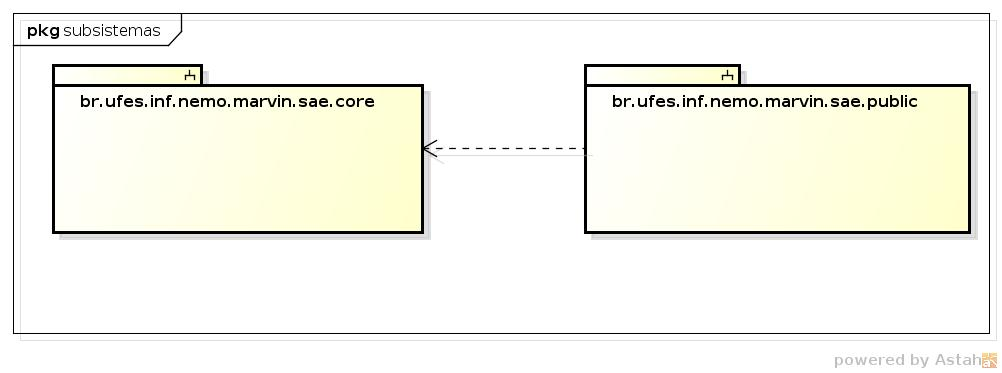
\includegraphics[width=1\textwidth]{figuras/fig-projeto-diagrama-pacotes}
  \caption{Diagrama de Pacotes e os Subsistemas Identificados.}
  \label{figura-subsistema}
\end{figure} 





\begin{table}[h]
	\centering	
	\vspace{0.5cm}
	
	\begin{tabular}{|p{3cm}|p{12cm}|}  \hline \rowcolor[rgb]{0.8,0.8,0.8}
	
 		Subsistema & Descrição \\\hline 
 		                             
		Core & Envolve toda a funcionalidade relacionada com o administrador do sistema, abrangendo controle de Séminarios, Cursos, Assuntos de interesse, envio de email automático e pré-cadastro de egresso. \\\hline
		                              
		Public & Envolve toda a funcionalidade relacionada com consultas a serem realizadas no site, e com as interações que os egressos poderão fazer, tais como cadastrar depoimentos e sugestões. \\\hline 
		
	\end{tabular}
	\caption{ Subsistemas}	
\end{table}


\chapter{Modelo de Casos de Uso}
\label{sec-caso-de-uso}

\newcounter{uccount}                                      \renewcommand*\theuccount{UC-\arabic{uccount}}
\newcommand*\UC{\refstepcounter{uccount}\theuccount}      \setcounter{uccount}{0}

O modelo de casos de uso visa capturar e descrever as funcionalidades que um sistema deve prover para os atores que interagem com o mesmo. Os atores identificados no contexto deste projeto estão descritos na tabela~\ref{tabela-atores}.

\begin{table}[h]
	\centering \vspace{0.5cm} \caption{ Atores}
	\begin{tabular}{|p{3cm}|p{12cm}|} \hline \rowcolor[rgb]{0.8,0.8,0.8}
 		Ator & Descrição \\\hline                              
		Administrador & Profissional da Ufes responsável pela parte administrativa do sistema. \\\hline   
		Coordenador & É um administrador responsável por um curso, avaliando depoimentos e sugestões enviadas pelos egressos. \\\hline                              
		Egresso & Ex-alunos da Ufes que tenham se formado em algum curso oferecido pelo DI/Ufes. \\\hline                              
		Visitante & Qualquer pessoa que acessar o site. \\\hline 		 
	\end{tabular}
	\label{tabela-atores}	
\end{table}



A Figura~\ref{figura-caso-de-uso-atores} apresenta o diagrama de herança entre os atores do sistema, de modo que essas heranças não serão mostradas nos outros diagramas para evitar a poluição visual.

\begin{figure}[h!]
	\centering
	\includegraphics[width=0.5\textwidth]{figuras/atoresHeranca}
 	\caption{Diagrama de Herança dos Atores.}
 	\label{figura-caso-de-uso-atores}
\end{figure}


A seguir, são apresentados os diagramas de casos de uso e descrições associadas, organizados por subsistema.


\newpage
\section{Subsistema Core}

A Figura~\ref{figura-caso-de-uso-core} apresenta o diagrama de casos de uso do subsistema Core.

\begin{figure}[h!]
	\centering
	\includegraphics[width=1\textwidth]{figuras/casodeuso-core}
 	\caption{Diagrama de Casos de Uso do Subsistema Core.}
 	\label{figura-caso-de-uso-core}
\end{figure}
 
 A seguir, são apresentadas as descrições de cada um dos casos de uso identificados. Os casos de uso cadastrais de baixa complexidade, envolvendo inclusão, alteração, consulta e exclusão, são descritos na tabela~\ref{tabela-core-cadastrais}.


\newpage
\begin{table}[h]
	\centering  \vspace{0.5cm} 	\footnotesize 
	\caption{Casos de Uso Cadastrais}
	\begin{tabular}{|c|c|c|p{6cm}|c|c|} \hline  \rowcolor[rgb]{0.8,0.8,0.8}
 				
 		Id & Nome  &  Ações  &  Observações & Requisitos   & Classes  \\ 	\hline \hline	
 		
 		{}    &    {}    &   I   &    Informar: nome, email, matricula e CPF. Será criada uma senha padrão, e assim que o administrador fizer o primeiro acesso, o sistema solicitará a atualização da mesma.  &   {}   &   {}    \\\cline{3-4}
 		{}  &   Gerenciar    &   A   &   {}   &    {}   &    {}  \\ \cline{3-4}
 		\UC\label{uc-administrador}  &  Administradores  &  C  &   {}    &   RF-1  &   Administrador    \\\cline{3-4}
 	    {}   &  {}   &    E    &    Não é permitido excluir um administrador que é coordenador de um curso.   &  {}  &  {} \\ \hline \hline
 		
 		
 		
 		\rowcolor[rgb]{0.97,0.97,0.97}
 		{}   &  {}   &  I  &   Informar: nome, código e coordenador (deve ser escolhido dentre os administradores cadastrados).   &  {}   &  {}    \\ \cline{3-4} \rowcolor[rgb]{0.97,0.97,0.97}
 		{} &   Gerenciar   &   A   &   {}   &    {}  &    {}   \\ \cline{3-4} \rowcolor[rgb]{0.97,0.97,0.97}
 		\UC\label{uc-curso} &    Cursos   &  C  &  {}  &  RF-3  &  Curso \\ \cline{3-4} \rowcolor[rgb]{0.97,0.97,0.97} 
 		{}    &    {}     &   E   &    Não é permitido excluir um curso que tenha egressos associados.  &  {}   & {} \\ \hline \hline
 		  
 		  
 		  
 		          
 		{}     &   {}    &   I   &    Informar: nome.     &   {}   &    {}    \\ \cline{3-4}
 		{}  &   Gerenciar   &   A   &   {}      &   {}    &    Assunto de   \\\cline{3-4}
 		\UC\label{uc-assunto}  &    Assuntos de   &    C   &    {}     &  RF-4  &    Interesse   \\\cline{3-4}
 		{} & interesse & E & Não é permitido excluir um assunto que tenha seminários associados. & {} & {} \\ \hline \hline
 		
 		
 		
 		\rowcolor[rgb]{0.97,0.97,0.97}
 		{} & {} & {} & Informar: nome, email, CPF, data de nascimento, identidade, sexo, naturalidade e nacionalidade. & {} & {} \\ \rowcolor[rgb]{0.97,0.97,0.97} 
 		{} & Gerenciar  &  I  & O sistema ao registrar o egresso  &  RF-2  &  Egresso,   \\  \rowcolor[rgb]{0.97,0.97,0.97}
 		\UC\label{uc-egresso}  & Egressos  &  {}   &  deve enviar um email para o mesmo.  &  RF-6   &    {}     \\ \cline{3-4} \rowcolor[rgb]{0.97,0.97,0.97}
 		{}  &  {}   &  A  &   {}    &  RN-1 &    Curso Realizado   \\\cline{3-4} \rowcolor[rgb]{0.97,0.97,0.97}
 		{}  &  {}   &  C  &   {}    &   RF-7   &    {}   \\\cline{3-4} \rowcolor[rgb]{0.97,0.97,0.97}
 		{}  &  {}   &  E  &   Não é permitido excluir egressos.   &  {}   &  {}  \\ \hline \hline
 		
 		
 		
		{}  &  {}  &  I  &  Informar: titulo, palestrante, data, local e assunto de interesse.  &  {}  &  {}  \\ \cline{3-4}
 		{} & {}  &  A  &  Caso o seminário já tenha sido confirmado e enviado email, o sistema deve enviar um email aos egressos informandos as alterações. & {} & {} \\ \cline{3-4}
 		\UC\label{uc-seminario}   &  Gerenciar   &    C   &    {}     &  RF-5   &    Seminário   \\ \cline{3-4}
 		{}    &    Seminários   &  E  &  Caso o seminário já tenha sido confirmado e enviado email, o sistema deve enviar um email aos egressos informandos a exclusão do seminário.  &  {}   &  {}   \\ \hline 
 		 		
 		 		
	\end{tabular}
	\label{tabela-core-cadastrais}
\end{table}




\newpage
\begin{flushright}    \textbf{Descrição de Caso de Uso}   \end{flushright}         
\noindent  \textbf{Projeto:} \imprimirtitulo  \\ 
\textbf{Identificador do Caso de Uso:} \UC\label{uc-seminario} \\ 
\textbf{Caso de Uso:} Confirmar Seminário e Convidar Palestrante \\
\noindent \textbf{Descrição Sucinta:} Este caso de uso é responsável por confirmar a ocorrência de seminários e por convidar egressos para se apresentarem como palestrantes.\\

\begin{table}[h]
	\centering    \vspace{0.5cm}     \footnotesize
	\caption{Fluxos de Eventos Normais}
	\begin{tabular}{|p{2.3cm}|p{1.8cm}|p{10.7cm}|} \hline  \rowcolor[rgb]{0.8,0.8,0.8}
 					
 		Nome do Fluxo & Precondição & Descrição  \\ \hline		
		
		Confirmar & {} & 1. O administrador informa o seminário a ser confirmado.  \\
		Seminário & {} & 2. O sistema envia email a todos os egressos que tenham interesse naquele assunto.\\ \hline 
			
		Convidar & {} & 1. O administrador informa o seminário sem palestrante.  \\
		Palestrante & {} & 2. O sistema envia email a todos os egressos que tenham interesse naquele assunto, convidando-os a serem o palestrante.\\ \hline 
		
		
		Voluntariar & {} & 1. O egresso informa o assunto e voluntaria-se como palestrante.  \\
		Palestrante & {} & 2. O sistema envia um email para informar o administrador.\\ \hline 
		
	\end{tabular}	
\end{table}

	\begin{table}[h]
		\centering 	\vspace{0.5cm}    \footnotesize
		\caption{Fluxos de Eventos Variantes}
		\begin{tabular}{|p{4.3cm}|p{3.5cm}|p{7.0cm}|}    \hline  \rowcolor[rgb]{0.8,0.8,0.8}
 		
 			Fluxo Relacionado &  Variante  &  Descrição    \\	\hline		
		
			Voluntariar Palestrante/  & 2 - O envio de email      & 2a - O sistema envia um email para o usuário   \\ 
			Confirmar Seminário / 	  & retorna um erro.			&  que instalou o sistema informando do erro. \\
			Convidar Palestrante     &{}              & 3 - O sistema retorna uma mensagem de erro ao usuário. \\\hline
		
		\end{tabular}
	\end{table}	
	
	

\noindent  \textbf{Requisitos Relacionados:} RF-5, RF-16     \\ \textbf{Classes Relacionadas:} Seminário. 





\newpage
\begin{flushright}    \textbf{Descrição de Caso de Uso}   \end{flushright} 
\noindent \textbf{Projeto:} \imprimirtitulo \\
\textbf{Identificador do Caso de Uso:} \UC\label{uc-email-atualizar-dados}\\ 
\textbf{Caso de Uso:} Enviar email atualizar dados \\
\noindent \textbf{Descrição Sucinta:} Este caso de uso é responsável enviar para os egressos a cada 2 anos um email solicitando a atualização de seus dados.\\

\begin{table}[h]
	\centering 	\vspace{0.5cm} 	\footnotesize
	\caption{Fluxos de Eventos Normais}
	\begin{tabular}{|p{2.3cm}|p{1.1cm}|p{11.4cm}|} \hline  \rowcolor[rgb]{0.8,0.8,0.8}
 					
 		Nome do Fluxo & Precond. & Descrição  \\ \hline		
	
		Enviar email & {} & 1. O sistema verifica se o último pedido de atualização tem mais de 2 anos. \\ 
		
		{} & {} & 2. O administrador sendo alertado pelo sistema, envia email a todos o egressos. \\ \hline
		
		
				
	\end{tabular}	
\end{table}


	\begin{table}[h]
		\centering 	\vspace{0.5cm}    \footnotesize
		\caption{Fluxos de Eventos Variantes}
		\begin{tabular}{|p{3.8cm}|p{4cm}|p{7.0cm}|}    \hline  \rowcolor[rgb]{0.8,0.8,0.8}
 		
 			Fluxo Relacionado &  Variante  &  Descrição    \\	\hline		
		
			Enviar  		& 2 - O envio de email      & 2a - O sistema envia um email para o usuário   \\ 
			email		& retorna um erro.			&  que instalou o sistema informando do erro. \\
			{}    		&{}              			& 3 - O sistema retorna uma mensagem de erro ao usuário. \\\hline
		
		\end{tabular}
	\end{table}	

\noindent  \textbf{Requisitos Relacionados:} RF-12   %  \\ \textbf{Classes Relacionadas:} 












\newpage
\section{Subsistema Public}

A Figura~\ref{figura-caso-de-uso-public}  apresenta o diagrama de casos de uso do subsistema Public.

\begin{figure}[h!]
  \centering
  \includegraphics[width=1\textwidth]{figuras/casodeuso-public.jpg}
  \caption{Diagrama de Casos de Uso do Subsistema Public.}
  \label{figura-caso-de-uso-public}
\end{figure} 


Os casos de uso cadastrais de baixa complexidade, envolvendo inclusão, alteração, consulta e exclusão, são descritos na tabela~\ref{tabela-public-cadastrais}.

\begin{table}[h]
	\centering  \vspace{0.5cm} 	\footnotesize 
	\caption{Casos de Uso Cadastrais}
	\begin{tabular}{|c|c|c|p{6cm}|c|c|} \hline  \rowcolor[rgb]{0.8,0.8,0.8}
 				
 		Id & Nome  &  Ações  &  Observações & Requisitos   & Classes  \\ 	\hline 
 		
 		{}    &    {}    &   I   &    Informar: titulo, ano, intituição, estado e o país.  &   {}   &   {}    \\\cline{3-4}
 		\UC\label{uc-escolaridade}  &   Gerenciar    &   A  , C   &   {}   &    RF-14   &    Escolaridade  \\ \cline{3-4}
 		{}  & Escolaridades  &  E  &   {}    &   {}  &   {}  \\ \hline 
 		
 		{}    &    {}    &   I   &    Informar: faixa salarial, area de atuação, se atua na area de formação, o nível de escolaridade e se reside no Espirito Santo .  &   {}   &     \\\cline{3-4}
 		\UC\label{uc-historico}  &   Gerenciar    &   A  , C   &   {}   &    RF-14   &  Histórico      \\ \cline{3-4}
 		{}  & Histórico   &  E  &   {}    &   {}  &   do Egresso  \\ \hline 
 		
	\end{tabular}
	\label{tabela-public-cadastrais}
\end{table}




\newpage
Os casos de uso de consulta mais abrangente que as consulta a um único objeto, mas ainda de baixa complexidade, estão descritos na tabela~\ref{tabela-public-consulta}.

\begin{table}[h]
	\centering  \vspace{0.5cm} 	\footnotesize 
	\caption{Casos de Uso de Consulta}
	\begin{tabular}{|c|c|p{8cm}|c|c|} \hline  \rowcolor[rgb]{0.8,0.8,0.8}
 				
 		Id & Nome   &  Observações & Requisitos   & Classes  \\ 	\hline	
 		
 		{}  &  {}  &   As consultas aos egressos poderão ser feitas de forma  & {}   & {}    \\ 
 		{} &  Consultar   & geral onde serão mostrado todos os egressos, ou por  & {} & {} \\ 
 	    \UC\label{uc-consulta-todos-egresso}  &  Todos  & curso onde serão mostrados apenas os egressos que  & RF-13 & Egresso \\	
 	    {}  &  Egressos   &  formaram naquele curso, será exibido na tela para ao usuário o nome do egresso, o curso que realizou, o ano de inicio e o ano de termino.   & {}   & {}  \\	\hline
 	    
 	    
 	    
 	    {} &  {}  &  As consultas aos depoimentos poderão ser realizadas   & {}   & {}    \\ 
 		{} &  Consultar & de forma geral onde serão mostrados todos os  & {} & {} \\ 
 	    \UC\label{uc-consulta-depoimento} & Depoimento & depoimentos, ou por curso onde serão mostrados & RF-17 & Depoimento \\	
 	    {} & {}  & apenas depoimentos sobre o curso escolhido, será exibido na tela o conteúdo, o autor e a data de postagem. & {} & {} \\	\hline
 	    
 	     				
	\end{tabular}
	\label{tabela-public-consulta}
\end{table}




\newpage
\begin{flushright}    \textbf{Descrição de Caso de Uso}   \end{flushright}         
\noindent \textbf{Projeto:} \imprimirtitulo  \\
\textbf{Identificador do Caso de Uso:} \UC\label{uc-seminario} \\
\textbf{Caso de Uso:} Consultar dados Estatísticos \\
\noindent \textbf{Descrição Sucinta:} Este caso de uso é responsável por gerar relatórios com dados estatísticos sobre o perfil dos egressos.\\

\begin{table}[h]
	\centering \vspace{0.5cm} \footnotesize
	\caption{Fluxos de Eventos Normais}
	\begin{tabular}{|p{2.3cm}|p{1.8cm}|p{10.7cm}|} \hline  \rowcolor[rgb]{0.8,0.8,0.8}
 					
 		Nome do Fluxo & Precondição & Descrição  \\ \hline		
					
		Gerar    & {} & 1. O visitante informa o curso.  \\
		relatório    & {} & 2. O visitante informa o tipo de relatório: faixa salarial, atuação, escolaridade, entre outros (vide Documento de Especificação de Requisitos, seção 3.1).\\ 
        {} & {} & 3. O sistema gera o gráfico e mostra ao visitante.\\	\hline 
				
	\end{tabular}
\end{table}

\noindent  \textbf{Requisitos Relacionados:} RF-13       \\ \textbf{Classes Relacionadas:} Egresso, Histórico do Egresso.





\newpage
\begin{flushright}    \textbf{Descrição de Caso de Uso}   \end{flushright} 
\noindent \textbf{Projeto:} \imprimirtitulo \\
\textbf{Identificador do Caso de Uso:} \UC\label{uc-sugestao}\\ 
\textbf{Caso de Uso:} Gerenciar Sugestões \\
\noindent \textbf{Descrição Sucinta:} Este caso de uso é responsável gerenciar as sugestões enviadas pelos egressos.\\

\begin{table}[h]
	\centering 	\vspace{0.5cm} 	\footnotesize
	\caption{Fluxos de Eventos Normais}
	\begin{tabular}{|p{2.3cm}|p{1.8cm}|p{10.7cm}|} \hline  \rowcolor[rgb]{0.8,0.8,0.8}
 					
 		Nome do Fluxo & Precondição & Descrição  \\ \hline		
	
		Incluir nova  & {} & 1. O egresso informa o conteúdo da sugestão e o curso. \\ 
		Sugestão & {} & 2. O sistema preenche os campos data e autor. \\
		{} & {} & 3. O sistema envia um email ao coordenador do curso, informando da sugestão. \\ \hline
		
		Responder  & {} & 1. O coordenador seleciona a sugestão. \\ 
		Sugestão & {} & 2. O coordenador informa a resposta. \\
		{} & {} & 3. O sistema envia um email ao egresso autor da sugestão, com a resposta do coordenador. \\ \hline
				
	\end{tabular}	
\end{table}

\noindent  \textbf{Requisitos Relacionados:} RF-8, RF-11       \\ \textbf{Classes Relacionadas:} Sugestão










\newpage
\begin{flushright}    \textbf{Descrição de Caso de Uso}   \end{flushright} 
\noindent \textbf{Projeto:} \imprimirtitulo \\
\textbf{Identificador do Caso de Uso:} \UC\label{uc-depoimento}\\ 
\textbf{Caso de Uso:} Gerenciar Depoimentos \\
\noindent \textbf{Descrição Sucinta:} Este caso de uso é responsável gerenciar os depoimentos enviados pelos egressos.\\

\begin{table}[h]
	\centering 	\vspace{0.5cm} 	\footnotesize
	\caption{Fluxos de Eventos Normais}
	\begin{tabular}{|p{2.3cm}|p{1.8cm}|p{10.7cm}|} \hline  \rowcolor[rgb]{0.8,0.8,0.8}
 					
 		Nome do Fluxo & Precondição & Descrição  \\ \hline		
	
		Incluir novo & {} & 1. O egresso informa o conteúdo, se é anônimo e o curso. \\ 
		Depoimento & {} & 2. O sistema preenche os campos data e autor. \\
		{} & {} & 3. O sistema envia um email ao coordenador do curso, informando de um depoimento pendente. \\ \hline
		
		Avaliar  & {} & 1. O coordenador seleciona o depoimento pedente. \\ 
		Depoimento & {} & 2. O coordenador informa se liberado ou não liberado. \\\hline
				
		Alterar  & {} & 1. O egresso seleciona o depoimento. \\ 
		Depoimento & {} & 2. O egresso informa os novos dados. \\
		{} & {} & 3. O sistema envia um email ao coordenador do curso, informando de um depoimento pendente. \\ \hline
		
		Excluir   & {} & 1. O egresso seleciona o depoimento. \\ 
		Depoimento & {} & 2. O egresso confirma a exclusão. \\
		{} & {} & 3. O sistema exclui o depoimento. \\ \hline
				
	\end{tabular}	
\end{table}

\begin{table}[h]
	\centering 	\vspace{0.5cm}    \footnotesize
	\caption{Fluxos de Eventos Variantes}
	\begin{tabular}{|p{2.3cm}|p{4.8cm}|p{7.7cm}|}    \hline  \rowcolor[rgb]{0.8,0.8,0.8}
 		
 		Fluxo Relacionado &  Variante  &  Descrição    \\	\hline		
		
		Avaliar    & 2 - O coordenador avaliar como   & 2a - O sistema envia um email para o egresso,  \\ 
		Depoimento & não liberado & informando para refazer seu depoimento. \\\hline
		
	\end{tabular}
\end{table}

\noindent  \textbf{Requisitos Relacionados:} RF-9, RF-10     \\ \textbf{Classes Relacionadas:} Depoimento










\chapter{Modelo Estrutural}
\label{sec-modelo-estrutural}

O modelo conceitual estrutural visa capturar e descrever as informações (classes, associações e atributos) que o sistema deve representar para prover as funcionalidades descritas na seção anterior. A seguir, são apresentados os diagramas de classes de cada um dos subsistemas identificados no contexto deste projeto. Na seção~\ref{sec-dicionario} – Dicionário de Projeto – são apresentadas as descrições das classes, atributos e operações presentes nos diagramas apresentados nesta seção.


\section{Subsistema Core}

A Figura~\ref{figura-core-classe} apresenta o diagrama de classes do subsistema Core.

\begin{figure}[h]
  \centering
  \includegraphics[width=1\textwidth]{figuras/diagrama-classe-core}
  \caption{Diagrama de Classes do Subsistema Core.}
  \label{figura-core-classe}
\end{figure} 


\newpage

\section{Subsistema Public}


A Figura~\ref{figura-public-classe} apresenta o diagrama de classes do subsistema Public.

\begin{figure}[h]
  \centering
  \includegraphics[width=1\textwidth]{figuras/diagrama-classe-public.jpg}
  \caption{Diagrama de Classes do Subsistema Public.}
  \label{figura-public-classe}
\end{figure} 
\newpage



\chapter{Modelo Dinâmico}
\label{sec-modelo-dinamico}

O modelo dinâmico visa capturar o comportamento dinâmico do sistema. A seguir, são
apresentados os diagramas de estados e o diagrama de atividades elaborados no contexto deste
projeto.


\section{Diagramas de Estados}


A Figura~\ref{figura-estado-depoimento} apresenta o diagrama de estados da classe Depoimento do subsistema Public.

\begin{figure}[h]
  \centering
  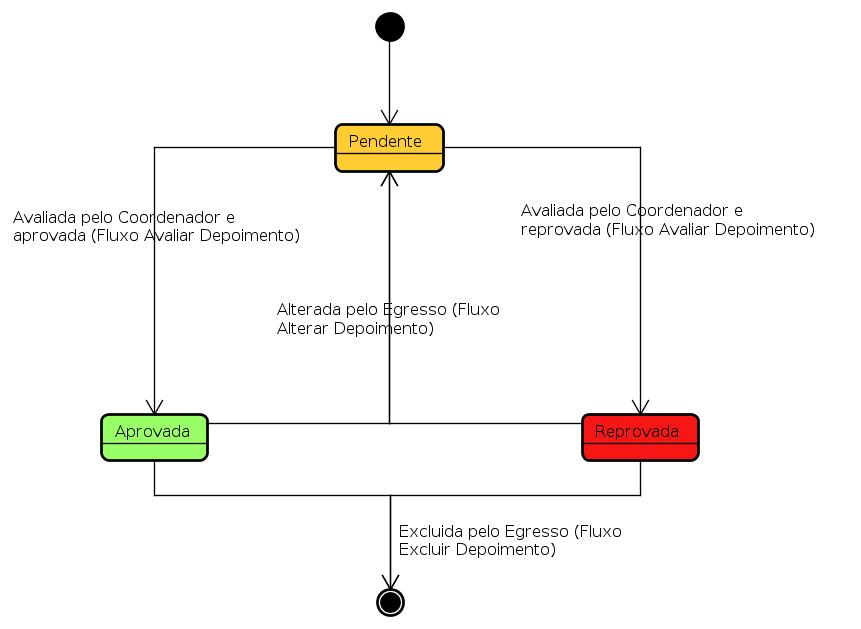
\includegraphics[scale=0.45]{figuras/estado-depoimento.jpg}
  \caption{Diagrama de Estados da Classe Depoimento.}
  \label{figura-estado-depoimento}
\end{figure}


\chapter{Dicionário de Projeto}
\label{sec-dicionario}
\setcounter{table}{0}

Esta seção apresenta as definições das classes (e seus atributos), servindo como um glossário do projeto. As definições são organizadas por subsistema. Vale destacar que eventuais operações que estas classes vierem a ter não são listadas e descritas nesta fase do projeto.


\section{Classes}

%%%%%       CLASSE EGRESSO        %%%%%%%%%%%%%%%%%%%%%%%%%%%%%%%%%%%%%%%%%%
\subsection{Egresso} \label{Egresso}
\begin{table}[h!]
	\footnotesize
	\begin{tabular}{|p{2.6cm}|c|c|p{7.8cm}|}   \hline \rowcolor[rgb]{0.8,0.8,0.8}
		
		%\multicolumn{4}{|c|}{ \textbf{Egresso}} \\ \hline \rowcolor[rgb]{0.95,0.95,0.95}
 		
 		\textbf{Propriedade} & \textbf{Tipo} & \textbf{Obrigatório?} & \centerline{\textbf{Descrição}} \\\hline  
 		                            
		nome & Texto & x & Nome completo do egresso. \\\hline  	
		
		data-nascimento & Data & x & Data de nascimento do egresso. \\\hline	
 		
		sexo & Caractere & x & Sexo do egresso. \\\hline 
		
		email & Texto & x & Email do egresso. \\\hline
		
		senha & Texto & x & Senha do egresso. \\\hline
		                             
		identidade & Texto & x & Número de RG do egresso. \\\hline
		
		cpf & Texto & x & Número de CPF do egresso. \\\hline
		
		naturalidade & Texto & & Naturalidade do egresso. \\\hline
		
		nacionalidade & Texto & & Nacionalidade do egresso. \\\hline
		
	\end{tabular}	
\end{table}


%%%%%       CLASSE EGRESSO-HISTORICO        %%%%%%%%%%%%%%%%%%%%%%%%%%%%%%%%%%%%%%%%%%
\subsection{Histórico do Egresso} \label{Histórico-do-Egresso}
\begin{table}[h!]
	\footnotesize
	\begin{tabular}{|p{2.6cm}|c|c|p{7.8cm}|}   \hline \rowcolor[rgb]{0.8,0.8,0.8}
	
		%\multicolumn{4}{|c|}{ \textbf{Histórico do Egresso}} \\ \hline \rowcolor[rgb]{0.95,0.95,0.95}
		
 		\textbf{Propriedade} & \textbf{Tipo} & \textbf{Obrigatório?} & \centerline{\textbf{Descrição}} \\\hline  	
	
 		data-envio & Data & x & Data de envio dos dados pelo egresso. \\\hline
		                      
		faixa-salarial & Enumerado & x & Faixa onde se encontra a renda do egresso. \\\hline
		
		area-atuacao & Enumerado & x & Área onde o egresso atua profissionalmente. \\\hline
		
		escolaridade & Enumerado & x & Nível de escolaridade do Egresso. \\\hline
		
		atua-na-area & Booleano & x & Se o egresso atua na área em que se formou. \\\hline		
		
		reside-ES & Booleano & x & Se o egresso reside no estado do Espirito Santo. \\\hline	
			
	
	\end{tabular}	
\end{table}


%%%%%       CLASSE ESCOLARIDADE        %%%%%%%%%%%%%%%%%%%%%%%%%%%%%%%%%%%%%%%%%%
\subsection{Escolaridade} \label{Escolaridade}
\begin{table}[h!]
	\footnotesize
	\begin{tabular}{|p{2.6cm}|c|c|p{7.8cm}|}   \hline \rowcolor[rgb]{0.8,0.8,0.8}
	
		%\multicolumn{4}{|c|}{ \textbf{Escolaridade}} \\ \hline \rowcolor[rgb]{0.95,0.95,0.95}
		
 		\textbf{Propriedade} & \textbf{Tipo} & \textbf{Obrigatório?} & \centerline{\textbf{Descrição}} \\\hline  	
	
 		titulo & Enum & x & Titulo da graduação adiquirida. \\\hline
		
		estado & Texto & x & Nome do estado onde foi realizado. \\\hline   
 		                      
		país & Texto & x & Nome do país onde foi realizado. \\\hline
		
		ano & Data & x & Ano de conclusão. \\\hline
		
		instituição & Texto & x & Nome da instituição onde foi realizado. \\\hline	
		
			
		
	\end{tabular}	
\end{table}

\newpage

%%%%%       CLASSE CURSO        %%%%%%%%%%%%%%%%%%%%%%%%%%%%%%%%%%%%%%%%%%
\subsection{Curso} \label{Curso}
\begin{table}[h!]
	\footnotesize
	\begin{tabular}{|p{2.6cm}|c|c|p{7.8cm}|}   \hline \rowcolor[rgb]{0.8,0.8,0.8}
	
		%\multicolumn{4}{|c|}{ \textbf{Curso}} \\ \hline \rowcolor[rgb]{0.95,0.95,0.95}
		
 		\textbf{Propriedade} & \textbf{Tipo} & \textbf{Obrigatório?} & \centerline{\textbf{Descrição}} \\\hline 
 		                            
		nome & texto & x & Nome do curso. \\\hline 
		
		código & texto & x & Código do curso. \\\hline 
		                             
		
	\end{tabular}	
\end{table}



%%%%%       CLASSE ASSUNTO DE INTERESSE          %%%%%%%%%%%%%%%%%%%%%%%%%%%%%%%%%%%%%%%%%%
\subsection{Assunto de Interesse} \label{Assunto-de-Interesse}
\begin{table}[h!]
	\footnotesize
	\begin{tabular}{|p{2.6cm}|c|c|p{7.8cm}|}   \hline \rowcolor[rgb]{0.8,0.8,0.8}
	
		%\multicolumn{4}{|c|}{ \textbf{Assunto de Interesse }} \\ \hline \rowcolor[rgb]{0.95,0.95,0.95}
		
 		\textbf{Propriedade} & \textbf{Tipo} & \textbf{Obrigatório?} & \centerline{\textbf{Descrição}} \\\hline
 		                            
		nome & texto & x & Nome do assunto de interesse. \\\hline
		
		
		
	\end{tabular}	
\end{table}


%%%%%       CLASSE DEPOIMENTO          %%%%%%%%%%%%%%%%%%%%%%%%%%%%%%%%%%%%%%%%%%
\subsection{Depoimento} \label{Depoimento}
\begin{table}[h!]
	\footnotesize
	\begin{tabular}{|p{2.6cm}|c|c|p{7.8cm}|}   \hline \rowcolor[rgb]{0.8,0.8,0.8}
	
		%\multicolumn{4}{|c|}{ \textbf{Depoimento}} \\ \hline \rowcolor[rgb]{0.95,0.95,0.95}
		
		\textbf{Propriedade} & \textbf{Tipo} & \textbf{Obrigatório?} & \centerline{\textbf{Descrição}} \\\hline  	
 		                           
		conteudo & Texto & x & Conteúdo postado pelo egresso no depoimento. \\\hline
		  
  		data-envio & Data & x & Data de envio do depoimento. \\\hline 
  		
		anonimo & Booleano & x & Se o depoimento é anônimo. \\\hline  
		
		status & Enum & x & Status do depoimento. \\\hline 		
  		
	\end{tabular}	
\end{table}


%%%%%       CLASSE Sugestao          %%%%%%%%%%%%%%%%%%%%%%%%%%%%%%%%%%%%%%%%%%
\subsection{Sugestao} \label{Sugestao}
\begin{table}[h!]
	\footnotesize
	\begin{tabular}{|p{2.6cm}|c|c|p{7.8cm}|}   \hline \rowcolor[rgb]{0.8,0.8,0.8}
	
		%\multicolumn{4}{|c|}{ \textbf{Sugestao}} \\ \hline \rowcolor[rgb]{0.95,0.95,0.95}
		
 		\textbf{Propriedade} & \textbf{Tipo} & \textbf{Obrigatório?} & \centerline{\textbf{Descrição}} \\\hline
 		                            
		conteudo & texto & x & Conteúdo postado pelo egresso  na sugestão. \\\hline
		
		resposta & texto & {} & Resposta do coordenador para a sugestão do egresso. \\\hline
		  
  		data-envio & Data & x & Data de envio da sugestão. \\\hline 
  	
  		
	\end{tabular}	
\end{table}


%%%%%       CLASSE SEMINÁRIO          %%%%%%%%%%%%%%%%%%%%%%%%%%%%%%%%%%%%%%%%%%
\subsection{Seminário} \label{Seminário}
\begin{table}[h!]
	\footnotesize
	\begin{tabular}{|p{2.6cm}|c|c|p{7.8cm}|}   \hline \rowcolor[rgb]{0.8,0.8,0.8}
	
		%\multicolumn{4}{|c|}{ \textbf{Seminário}} \\ \hline \rowcolor[rgb]{0.95,0.95,0.95}
		
 		\textbf{Propriedade} & \textbf{Tipo} & \textbf{Obrigatório?} & \centerline{\textbf{Descrição}} \\ \hline
 		
		nome do palestrante & Texto & {} & Respónsavel por realizar o seminário. \\\hline
		  
  		data & Data/Hora & {} & Dia da realização do seminário. \\\hline 
  		
  		titulo & Texto & x & Título do seminário. \\\hline  
  		
  		local & Texto & {} & Local onde se realizará o seminário. \\\hline 
  		
  		confirmado & booleano & {} & se o seminário já foi confirmado. \\\hline 
  		
	\end{tabular}	
\end{table}

\newpage

%%%%%       CLASSE ADMINISTRADOR       %%%%%%%%%%%%%%%%%%%%%%%%%%%%%%%%%%%%%%%%%%
\subsection{Administrador} \label{Administrador}
\begin{table}[h!]
	\footnotesize
	\begin{tabular}{|p{2.6cm}|c|c|p{7.8cm}|}   \hline \rowcolor[rgb]{0.8,0.8,0.8}
	
		%\multicolumn{4}{|c|}{ \textbf{Administrador}} \\ \hline \rowcolor[rgb]{0.95,0.95,0.95}
		
 		\textbf{Propriedade} & \textbf{Tipo} & \textbf{Obrigatório?} & \centerline{\textbf{Descrição}} \\\hline  	
 		                            
		nome & texto & x & Nome completo do administrador. \\\hline 
		
		email & texto & x & Email do administrador. \\\hline 
		                             
		cpf & texto & x & Número do CPF do administrador. \\\hline 
		
		matricula & texto & x & Número da matricula do administrador na UFES. \\\hline 
		
		senha & texto & x & Senha para entrar no sistema. \\\hline 
		
	\end{tabular}	
\end{table}


%%%%%       CLASSE CURSO-REALIZADO       %%%%%%%%%%%%%%%%%%%%%%%%%%%%%%%%%%%%%%%%%%
\subsection{Curso Realizado} \label{Curso-Realizado}
\begin{table}[h!]
	\footnotesize
	\begin{tabular}{|p{2.6cm}|c|c|p{7.8cm}|}   \hline \rowcolor[rgb]{0.8,0.8,0.8}
	
		%\multicolumn{4}{|c|}{ \textbf{Curso Realizado}} \\ \hline \rowcolor[rgb]{0.95,0.95,0.95}
		
 		\textbf{Propriedade} & \textbf{Tipo} & \textbf{Obrigatório?} & \centerline{\textbf{Descrição}} \\\hline 
 		                            
		matricula & texto & x & Número da matrícula do egresso no curso realizado. \\\hline 
		
		ano de início & Data & x & Data de início do curso pelo egresso. \\\hline 
		                             
		ano de fim & Data & x & Data de conclusão do curso pelo egresso. \\\hline 
	
		
	\end{tabular}	
\end{table}


\newpage

\section{Tipos de Dados Específicos de Domínio}

\subsection{Area-Atuacao} \label{Area-Atuacao}
	
	\begin{itemize}[noitemsep]
		\item Áreas em que os egressos podem estar atuando. Tipo enumerado que pode assumir os seguintes valores:
		\begin{itemize}[noitemsep]
  			\item empreendedor
  			\item funcionário no setor público
  			\item funcionário no setor privado
  			\item professor
  			\item pesquisador
		\end{itemize}
	\end{itemize}



\subsection{Faixa-Salarial} \label{Faixa-Salarial}

	\begin{itemize}[noitemsep]
	  \item  Faixa salarial do egresso. Tipo enumerado que pode assumir os seguintes valores:
	  	\begin{itemize}[noitemsep]
	  		\item até 3 salários mínimos
	  		\item de 3 a 5 salários mínimos
	  		\item de 5 a 10 salários mínimos
	  		\item de 10 a 15 salários mínimos
	  		\item de 15 a 20 salários mínimos
	  		\item acima de 20 salários mínimos.
		\end{itemize}
	\end{itemize}



\subsection{Título de Escolaridade} \label{Escolaridade}

	\begin{itemize}[noitemsep]
  	\item Título do curso realizado pelo egresso. Tipo enumerado que pode assumir os seguintes valores:
  		\begin{itemize}[noitemsep]
  			\item Superior
  			\item Especialização
  			\item Mestrado
  			\item Doutorado
 	 		\item Pós-Doutorado
		\end{itemize}
	\end{itemize}




\subsection{Área de formação} \label{area-formacao}

	\begin{itemize}[noitemsep]
  	\item Relação da área em que o egresso se formação na Ufes com a que ele esta atuando. Tipo enumerado que pode assumir os seguintes valores:
  		\begin{itemize}[noitemsep]
  			\item Atua na Área
  			\item Atua em Área Correlatao
  			\item Atua em Área não Correlata
		\end{itemize}
	\end{itemize}




% Finaliza a parte no bookmark do PDF para que se inicie o bookmark na raiz e adiciona espaço de parte no sumário.
\phantompart

% Marca o início dos elementos pós-textuais.
\postextual

\phantompart
\printindex

% Fim do documento.
\end{document}

%\include{apendices/projeto}
\end{apendicesenv}


% Índice remissivo.
\phantompart
\printindex

% Fim do documento.
\end{document}
